\documentclass[12pt]{article}
\usepackage{cite}
\usepackage{graphicx}
\usepackage{setspace}
\usepackage{indentfirst}
\usepackage{listings}
\usepackage{mathpazo}
\usepackage[T1]{fontenc}
\linespread{1.6}
\begin{document}

%Title page

\begin{titlepage}
    \begin{center}
        
        \begin{doublespace}        
        \textbf{\Large Navigating Articles of News Websites With a Web Metrics Visualization}
        \vfill

        \vspace{2in}
        \textbf{\Large Alain Ibrahim} \\
		\vspace{2in}
        A Thesis in the Field of Information Technology \\
        for the Degree of Master of Liberal Arts in Extension Studies \\

        \vspace{.5in} 

        
        Harvard University \\
        \vspace {.4in}
        March 2015        

		\end{doublespace}        
        
        \vfill
         
    \end{center}
\end{titlepage}

%Abstract

\section{Abstract}

Current prominent web traffic analytics systems such as Google Analytics report traffic per website, given certain filtering criteria. Such systems are typically geared to system administrators who use the data to identify patterns and possibly assist management in strategy making. For news sites, this may mean analyzing the traffic on a news article and where most of the readers came from. The end users, however, will at best see metrics such as social likes and shares within the visited article. But, what if we could provide the end users a near real-time metrics map of the entire news site they are visiting? What if they could navigate based on traffic patterns, as opposed to having to follow the common front page layout specified by the news editors? This is what I built - a system that hooks into a Wordpress-based news website, captures the visitors' web metrics, and conveys the near real-time traffic through an interactive web-based visualization.
\newpage

\begin{singlespace}
\tableofcontents
\end{singlespace}

\vfill

\section{Thesis Project Description}
In 2015, the web of online media can be divided into 2 categories: News websites that contain facts about world events and social media sites that cover the ongoing conversations around these events. Before social media became ubiquitous, the news information flow was one-directional - with hardly any feedback from the site visitors. Now, visitors share articles on their online social properties such as Facebook and Twitter. Yet, what appears on the front page of one's favorite news site is set by the web news editorial team and can be influenced by the news station's political or business agenda. 

My goal in this thesis is to create a different way of seeing the news, using an interactive web visualization. The product is geared to site visitors that are curious in knowing how long an article was popular for and how interested the readers were when they read that article. At the same time, these measures can be visually compared between 2 articles for a relative analysis of popularity and reader level of interest. 

Different news stations use different web content management systems (WCMS). The system that I built hooks into a very common and open source WCMS - Wordpress. It then captures web metrics, and visualizes these metrics inside an interactive web-based visualization. The visualization targets site visitors but can be equally used by web admins. There are 3 main pieces of data I took interest in capturing: The number of hits to a an article, the amount of time spent reading an article, and the geographic location of the visitor. 

In the first stage, I created a database to house the web metrics that I wanted to capture. I then created a server-side library that can be included into any Wordpress-based website. This library hooked into my database and captured the hits' metadata against the given news site. Such metadata includes time of article visit, region of visitor, and timezone of visitor.  
I then built the "business logic" of the data and information that I wanted to capture. This includes algorithms that produced the refined data and metrics to be ultimately communicated to the end user.
This amounted to the final step of creating an interactive visualization that shows near real-time user web traffic in each of the registered articles of the connected news site.

The domain that I targeted is \textbf{online news media}. I captured the below data, as far back as 31 days:
\begin{itemize}
\item The number of visitor hits to a given article. Each hit is defined by a unique timestamp and IP address
\item The visitor's geographic location
\item The amount of time a visitor spent reading the article for a given hit
\end{itemize}

\newpage

\noindent The interactive visualization enabled 4 tasks:
\begin{enumerate}
\item \textbf{To compare articles' hits and reader attention spans for any period within the last month, given a select category}
\item \textbf{To preview each article's thumbnail, title, and excerpt}
\item \textbf{To contrast the geographic distribution of hits and attention of up to 2 articles}
\item \textbf{To navigate to the full article counterpart on the subject news website}
\end{enumerate}

\noindent{As for interactivity, the visualization enabled the following:}
\begin{itemize}
\item Hovering over article elements to preview the thumbnail, title, and excerpt of the body content
\item Clicking on an article element to display a table that shows the geographic distribution of the number of hits and attention span for that article
\item Filtering the data via a controls box. The controls box allows the user to select a desired news category, to filter by date range, and to toggle context-related settings 
\end{itemize}

The final product was geared towards the conventional news site structure, where categories are enumerated (e.g. sports, health, science, politics, etc.), and where articles are listed under their pertinent categories. \\

\noindent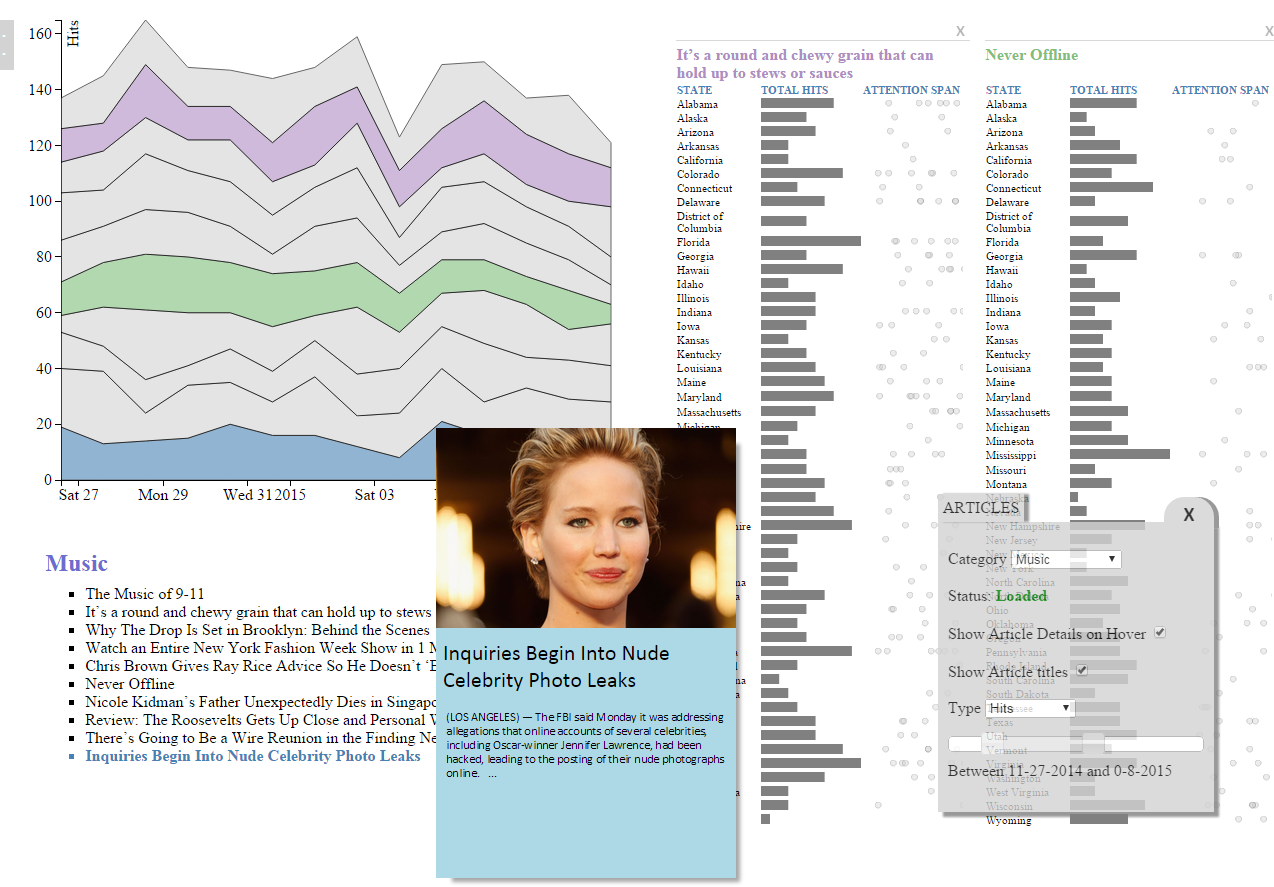
\includegraphics[scale=0.4]{img/in_action} \\

\begin{singlespace}
\noindent\textbf{Figure 1 -- The user previews a music article in the interactive visualization while having selected 2 articles for hits and attention span comparison.}
\end{singlespace}

\newpage

\noindent{Here are the technologies that I used in building my system:}
\begin{itemize}
\item MySQL for the relational database that houses the web metrics
\item PHP for the server-side script that stores and retrieves the data from the database
\item HTML 5 for laying out the basic components of the visualization - for example, the controls box
\item SVG to markup the visualization graph elements
\item CSS3 for styling the HTML and SVG elements
\item JavaScript to manipulate the DOM (Document Object Model) and to load data from the server side
\item D3.js (Data-Driven Documents) to facilitate the manipulation of the data in the visualization
\item jQuery to shorthand some lengthy JavaScript functions
\end{itemize}


%I built the system in the following chronological order:
%\begin{enumerate}
%\item Abstracted the web traffic data that needs to be captured and develop the business model. Specifically, I first defined what data was useful and how to develop the algorithms to capture it
%\item Built a relational database in MySQL around the results from 1)
%\item Developed server-side classes with PHP that captured and retrieved the collected data
%\item Researched and experimented with different visualizations that could best fit 2)
%\item Developed and implemented the client-side visualization using D3
%\end{enumerate}

\vfill

\section{Prior Work}
\subsection{Visualization}
Prominent researchers in the field of visualization have concocted logical constructs and approaches to designing and implementing quality visualizations. From a presentation standpoint, there is much emphasis on showing the end user just enough visual data for the user to achieve the intended task of the visualization - this is known as \textbf{expressiveness} (Schumann \& Muller, 2000) - where the visualization shows information only relevant to the data set. Another popular concept in visual economics is the \textbf{data-to-ink ratio} (Tufte, 2001). The goal is to have just enough ink presented to convey the data; additional ink that is not matched by data is a distraction. 

Having an efficient visualization is not enough. It needs to be effective. This brings us to two concepts covered in depth by Tamara Munzner: \textbf{domain} and \textbf{task} (Munzner, 2009). She advocates that in the design phase, the builder needs to identify the domain that he/she is working with. A domain is a world of ideas and concepts that are abstracted under one umbrella. For example, human anatomy, software engineering, economics, and biology are all domains. A domain gives rise to concepts, definitions, and a pre-built library of shapes and colors by the convention of collective knowledge. Red in biology signifies blood whereas in the world of novels it may allude to romance. Thus the target domain largely determines what colors and shapes the visual designers will have on their palette. \\
On the other hand, the task refers to the "what" of the visualization. What is/are the goal(s) of the visualization? Is it to explore, analyze, extrapolate, etc.? Clearly identifying the task(s) of the visualization at hand solidifies the direction in which the designer \textbf{encodes} the visual variables (Carpendale, 2003). Encoding refers to the idea of representing a quantitative or qualitative concept visually. The visual variables include position, size, shape, value, color, orientation, grain, and texture. For an effective visualization, the choice of encodes is dependent on the domain of the visualization, as well as the tasks the visualization aims to support. \\
Studies have shown that position and length are the easiest and fastest visual variables to decode (Cleveland \& McGill, 1984). My project deals with two main measures: Number of hits and read time (in seconds). To incorporate position, I can plot these two measures on a Cartesian graph with time on the X axis and the selected measure on the Y axis. If I plot each datum as a dot or cirle, I end up with a scatterplot. A scatterplot is essentially a plot of data - usually in the form or dots or circles - on a cartesian coordinates system. Though, my goal is show trends of popularity. When we think of trends we usually have a mental map of a connected sequence over time - which is why a line chart and area chart are better candidates as they convey patterns of over time, rather than scattered concentrations of data. \\
\noindent As for comparing the total number of hits across different geographic locations, we need to use another variable - length. Bar charts are great candidates for conveying magnitude and for contrasting magnitudes across different categories. Usually, bar charts are oriented vertically or horizontally. For our purpose, a horizontal bar chart suits the task, as it keeps the labels of the geographic origins from visually overlapping (Swires-Hennesy, 2014). Lastly, visualizing the number of seconds for each observation given a geographic location over a specified time period is best accomplished through the usage of position; for this, I can employ a dot chart. A dot chart is essentially a one-dimensional scatterplot. \\
For distinguishing categories in a line or graph chart, color is an effective visual variable. For this project, news categories are not simultaneously contrasted - but articles are. Encoding each article with a different color may work well for up to 5 colors; however, studies show that surpassing this limit makes it difficult for humans to differentiate encodes of more than 7-9 colors (Healey, 1996). Thus a different visual variable will need to be applied to effect in the visitor distinguishing the articles from one another. Here, I can resort to the visual variable of position. A stacked area graph is an area graph that employs position by stacking different parts of the whole on top of one another against another dimension - usually time (Byron \& Wattenberg, 2008).  

In the pre-Internet days, the implementation would have ended here. Though, with the advent of mass computerization and global connectivity, a new ability has been introduced - that of interactivity. Interactivity helps enable multiple views of the same data, using the same visualization. In visualization, interactivity has been broken down into the following: Overview+Detail, Zooming, Focus+Context, details-on-demand, and cue-based systems (Cockburn, Karlson, \& Bederson, 2008). The user is now able to manipulate the views of the data using input devices such as a mouse and keyboard. Here, I could support narrowing the selected time range by zooming, and retrieving the articles' previews through details-on-demand. 


\subsection{Measuring Time}
Time is an essential component to web analytics, as it gives context to what is being measured. Although graphing change over time was attempted in the early A.D.s, the first known contemporary time series graph was published by William Playfair (Playfair \& Corry, 1801). Playfair was the father of the line graph and bar graph. However, there is not a single model that accommodates all domains and tasks (Frank, 1998). Thus, for the proposed visualization, time must be dealt with in the context of an online news domain.   

Here, it is important to note the difference between event data and interval data (Wills, 2011). Time events are occurrences that are represented as slices of time; for example, a plane landed at its destination is an event. Whereas, the process of a plane landing occurs over a time interval of say 20 minutes. In this project, an article hit is defined as an event. That said, if I visualize time on an X axis it is inevitable that I will have units of time where no hits are available. The rendering of this time interval as a discrete event is adequate so long as the measured interval is minute compared to the total time covered by the data (Graham). That is, a visitor reading an article for 2 minutes is a small amount compared to say an article's lifetime of 3 weeks. Thus, plotting the observation as it being a slice of time is adequate.  

In order to have a better understanding of the time intervals of news, I asked professionals around the news station that I work at for feedback. Based on this and my observations of our news website and other similar entities' websites, "news" refers to a recent occurrence, notably something that happened today. "Breaking News" typically refers to an event that happened within the current day and whose story under development. "Recent News" pertains to stories created within the last 1-3 days. Most older news items are considered archives. \\
 My goal in this project is to represent the "recent news" category. Thus, the needed time granularities to be conveyed that support the task of the proposed visualization should be in days (Bettini, Jajodia, \& Wang, X. S., 2000). At a minimum for drilling down to a day's worth of news, I need to use a discrete time scale (Goralwalla, \"{O}zsu, \& Szafron, 1998) and thus need to capture the day, hour, and minute of each visit. The output variables connected to time should be the number of hits and the average read time spent on an article.

\newpage

\subsection{Existing web metrics systems}
What I built is novel in that there is no current navigable and exploratory tool for site visitors, which visualizes near real-time traffic on news sites. \\
Upon researching online, I came across a few systems that specialize in visualizing web metrics: \\

\noindent\textbf{Flow (http://www.webresourcesdepot.com/beautiful-free-website-traffic-visualization-application-flow/)} \\ \\
\noindent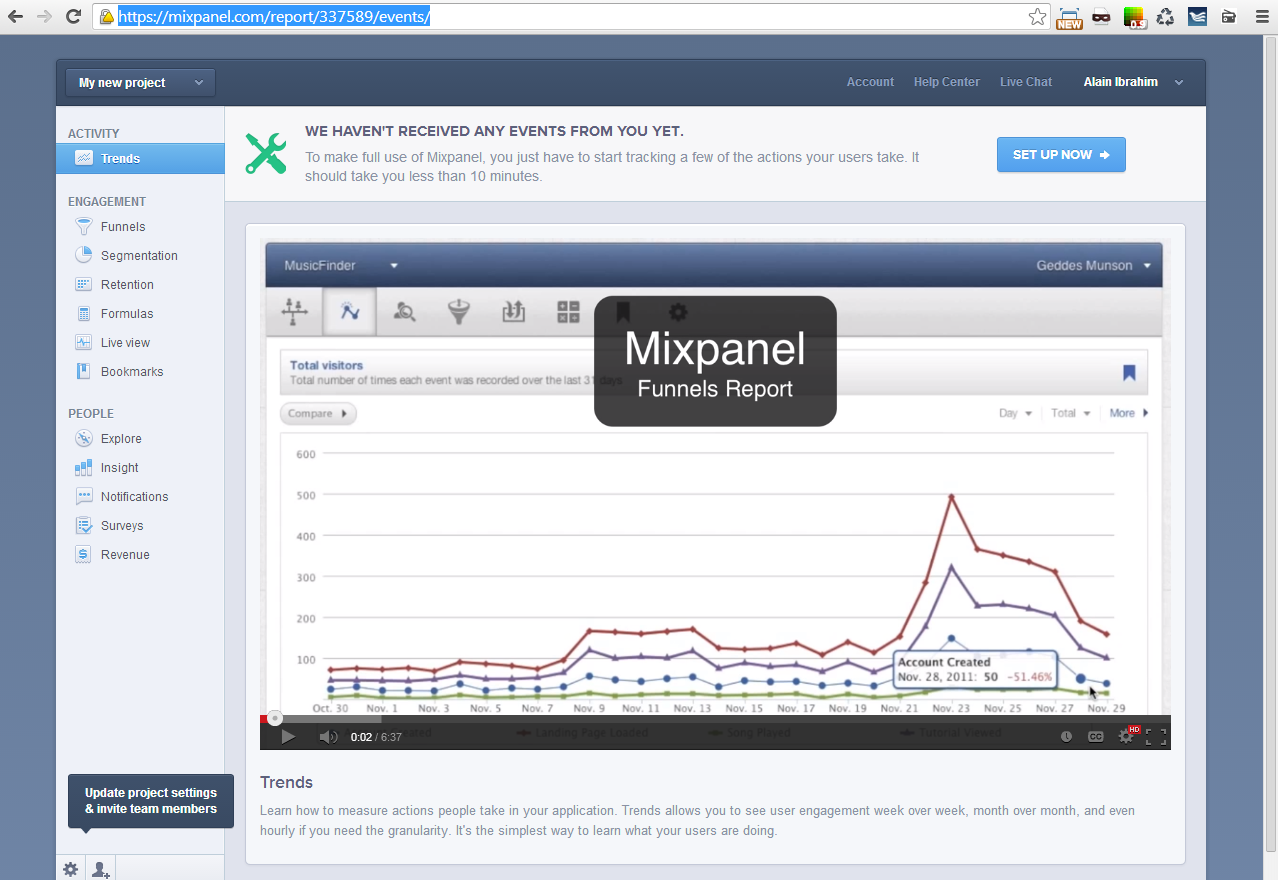
\includegraphics[scale=0.45]{img/flow}
\begin{singlespace}
\noindent\textbf{Figure 2 -- A line graph that measures the number of hits on the y axis, and date on the x axis for select categories on a given website.} \\
\end{singlespace}

While this can be useful in providing some feedback to the news site's administrators, it does not provide detailed insight to the articles in a given news site. The below screenshot demonstrates another visualization part of Flow. \\

\vfill

\noindent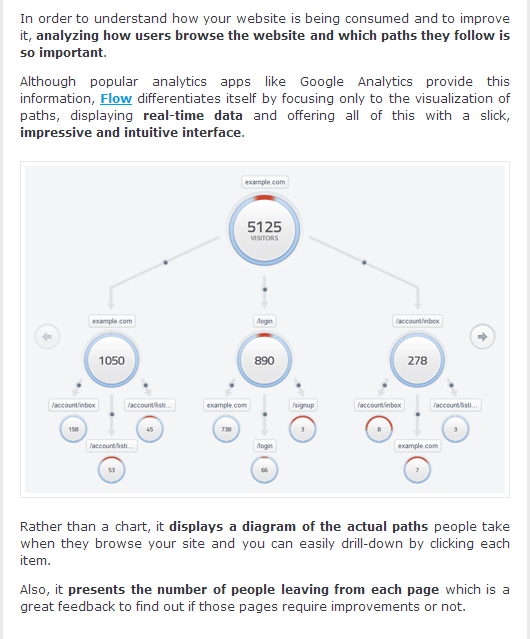
\includegraphics[scale=0.7]{img/flow1} \\
\noindent\textbf{Figure 3 -- Highlights of Flow.} \\

\newpage


\noindent\textbf{Google Analytics} \\ \\
\noindent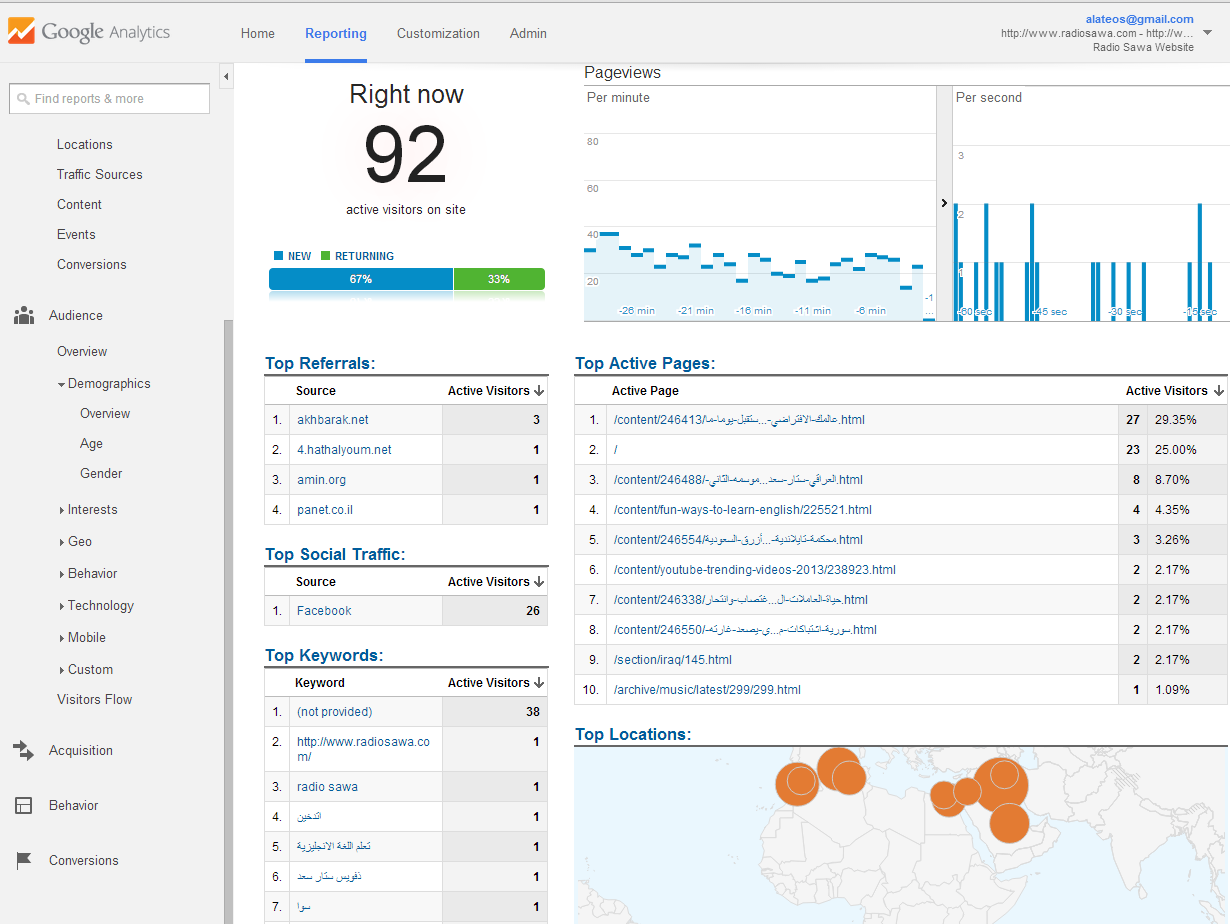
\includegraphics[scale=0.4]{img/google_analytics} \\
\noindent\textbf{Figure 4 -- The Real-Time metrics pane in Google Analytics.} \\

Google Analytics comes in handy in aggregating data and conveying statistical data to a site admin. The admin here would navigate with the intention of running an analysis, such as: From what parts of the world is most of this website's traffic coming from? What links are being most visited?
While this is a great tool for decision making, it is unlikely that the news site visitors will wake up to their coffee looking at this, and use it to navigate to the actual news website. \\

\newpage

\noindent\textbf{Adobe Analytics} \\


Adobe Analytics covers a slew of reporting capabilities:

\begin{itemize}
\item \textbf{Marketing reports and analytics.} Includes dashboards and reports, conveying key performance indicators, showing marketing strategies' performance in real-time, and displaying the results of ad campaigns
\item \textbf{Ad hoc analysis.} Includes multidimensional site analysis and advanced reporting
\item \textbf{Data workbench.} Involves collecting, processing, analyzing, and visualizing Big Data from online and offline customer interactions
\item \textbf{Predictive analysis.} Pertains to discovering hidden customer behavior
\item \textbf{Real-time web analytics.} Shows what is happening on the digital properties in real-time so that managers can take action where needed
\end{itemize}

Once again, the intended audience is that of management and decision makers. What I plan to create is something that the news consumers could see and use to make decisions on what to navigate to.

\null
\vfill


\section{Implementation - data capture}
\subsection{Capturing Data}
\subsubsection{IP Addresses}
Internet users access the Internet through their ISP (Internet Service Provider). The device that connects a user to the ISP is what is commonly known as a broadband router. This broadband router is uniquely identified by a series of numbers, called the "IP address". An IP address is a number that uniquely identifies any device that is connected to a network that uses the Internet Protocol. It is the means that I used to track a user and that does not require user authentication. The IP address that I was interested in capturing is the public IP address of the visitor's ISP (Internet Service Provider) router. 

An IP address can be static or dynamic. The former is set by the network administrator and remains in place unless it is changed manually. The latter is assigned by the network router, and is assigned for a temporary period called the DHCP lease time. After the period of the lease time has expired, the device is given a new IP address by the router. For this reason, I needed to ensure that this IP address did not renew so much as to violate the constraint set by the revisit threshold. The revisit threshold is a measurement setting which I created to determine whether enough time has passed for the next article hit to be counted as a new one. For example, if the revisit threshold is set to 5 minutes, and someone's IP address changes every 1 minute, then the user behind the IP address can visit an article several times within the 5-minute period and cause the metrics system to register 5 different hits - each from a different IP address - when it should just register 1 hit. Thus for the revisit threshold to work effectively, the IP address of the visitor must remain constant from the time stamp of the article hit, and until the time period specified by the revisit threshold has passed. \\
In order to obtain the average DHCP lease time set by routers, I resorted to a few network engineers and contacted 3 prominent ISPs (Internet Service Providers). Here are the results:
\vspace{0.3in}

\begin{tabular}{| c | c |}
  \hline                       
  Network Engineer 1 & 7 days \\[1ex] \hline
  Network Engineer 2 & 3 days \\[1ex] \hline
  Network Engineer 3 & 3 days \\ [1ex] \hline
  Verizon (ISP) & 14 days \\[1ex] \hline
  Comcast (ISP) & 4-7 days \\[1ex]
  \hline  
\end{tabular}
\vspace{0.3in}

The average DHCP lease time turned out between 3 and 7 days. The question then became, when should the next article hit be counted as a new one? People can visit the same article several times a day. Thus this threshold is set so as not to over-count the visits in the event someone tries to inflate the hits numbers by constantly refreshing the visited article. From a practical standpoint, I see this limit set to a number between 5 minutes and 1 hour. For this reason, it is safe to treat static and dynamic IP addresses the same - as the time revisit threshold is less than the average renew period of at least 1 day. This is important as I have defined a hit as a page view that is coming from a unique IP address.

\noindent There is a drawback using this method in that it categorizes all users behind an ISP router as the same one user. For example, if me and 3 people visited the same article in a period of 10 minutes, and if the revisit threshold was set to 10 minutes, then the code would count all of our visits as 1 hit. A more accurate way of counting each user would be to use a tracker on the client side, such as a cookie or HTML5's LocalStorage. Though, one can completely evade the system by respectively clearing the cookies and by disabling JavaScript. Therefore, a more accurate server-side hit counting method needs to be explored in the future.  

Capturing the hits required server-side scripting. In did this in PHP by storing the IP address of the visitor through the use of an associative array called \textbf{\$\_SERVER} that contains several variables pertaining to the HTTP connection between the client and the server. The variable that contains the IP address from which the user is viewing a select page is called \textbf{REMOTE\_ADDR}. In code, I registered the visiting IP address like so:
\begin{lstlisting}
$user_ip = $_SERVER["REMOTE_ADDR"];
\end{lstlisting}


As for user integrity, one cannot fully ensure that a physical human is sitting behind an IP address when automated scripts may be hitting the IP address of a given news article. Though, my goal was to minimize the inaccuracy when a visitor reached a news article. I countered this by registering the visiting IP address as soon as the user has moved his/her mouse, or, when he/she has scrolled at least once when viewing the article at hand. My thought was that moving a mouse or scrolling a screen mostly indicated the presence of a live being. \\ 
I tested this successfully in \textbf{register\_ip.php}. Here, I have a page containing several blocks of repeated Lorem ipsum text. I used JavaScript to listen to the mousemove and scroll events. I used jQuery to shorthand the event bindings. Below is the test code:
\begin{lstlisting}[basicstyle=\scriptsize]
mouse_moved = false;
page_scroll_counter = 0;

$("body").on("mousemove",function(){
	if(!mouse_moved) {
		\\ Here, a flag would be sent to the server via AJAX
		console.log("Mouse has moved");
		mouse_moved = true;
	} else {
		
	}
});

$(document).on("scroll",function(){
	if(page_scroll_counter == 1) {
		\\ Here a flag would be sent to the server via AJAX
		console.log("Page has been scrolled")
	} else {
		page_scroll_counter++
	}
});
\end{lstlisting}        

\newpage

\subsubsection{Geographic locations}
Another metric that I captured was the user geographic location distribution for a select news article. This required two steps:
\begin{enumerate}
\item Capturing the IP address of the user. This was demonstrated in the previous section
\item Obtaining the corresponding latitude and longitude coordinates associated with the user's IP address
\end{enumerate}

Here, it is important to note that many users may be sitting behind HTTP proxy servers. HTTP proxy servers are physical computers/servers that act as proxy points for the client computers. For example, if someone in Russia used a proxy server in the US to visit my news article, the requesting IP address that is captured is that of the US - making it appear that the user visited the article from the US. In PHP, in addition to \textbf{\$\_SERVER["REMOTE\_ADDR"]}, there is another variable called \\ \textbf{\$\_SERVER["HTTP\_X\_FORWARDED\_FOR"]}. While the former gets the IP address of the direct requester, the latter gets the originating IP that is making the request. So for example, if I were to be sitting behind an IP proxy server which had an address of 111.111.111.111, then \\ \$\_SERVER["REMOTE\_ADDR"] would carry that value. \\
In this case, \$\_SERVER["HTTP\_X\_FORWARDED\_FOR"] would then contain the value of my router's outside IP address - which is what I am looking to map geographically.   
\\ If on the other hand the user was browsing the Internet without the use of a proxy server, then \$\_SERVER["REMOTE\_ADDR"] would carry the value of the user's router's IP address - reflective of the user's geography; and, \$\_SERVER["HTTP\_X\_FORWARDED\_FOR"] would carry no value. \\ \\
\noindent Here is the methodology that used to capture the needed IP address for the geographic lookup:
\begin{enumerate}
\item Get the value of \$\_SERVER["REMOTE\_ADDR"] and look up its value with a geolocation API. Call this \textbf{X}
\item Get the value of \$\_SERVER["HTTP\_X\_FORWARDED\_FOR"] and look up its value with a geolocation API. Call this value \textbf{Y}
\item If X and Y are both available, it means that the user is sitting behind a proxy and that the needed IP address is that of Y. If X is available but Y is not, it means that Y is a private IP address of the device behind its router - and thus not behind a proxy server. In this case, X would hold the IP address of the origin.
\end{enumerate} 

The next step here was to find a service that would map a given IP address to its corresponding geo coordinates, and ideally to the originating region's name. A quick Google search revealed a convenient REST API service that outputs the responses in JSON. \textbf{Telize (www.telize.com)} is a REST API that allows developers to get the visitor IP address and to query the location information for that IP address. Such information includes the country of origin, region of origin, and timezone of origin. The upside of this service is that at the moment it contains to no rate limits; thus, one could make an indefinite amount of calls to the Telize API.

I tested the above code clause by visiting my test page from Alexandria, Virginia. When I did so without the use of a proxy server, the hit registered as coming from the United States. Then, when I set my Internet browser to use a proxy server in Brazil, the hit still registered as coming from the United States - as intended.

\subsubsection{Average Read Time}

Another metric that I was curious in attaining was how long the average user spent reading a certain news article. At the moment, a cousin measure called the bounce rate checks to see whether the user continues to browse other pages in the site, or whether the user 'bounces' off to other websites. Meaning, if I visited a certain website, I am tracked as to whether I visit several pages on that website or just bounce (leave) immediately. Leaving immediately results in a high bounce rate while visiting many pages on the visited site before leaving to another site results in a low bounce rate. 
Although this measure reflected the interest of the visitor has in the visited site overall, it did not indicate how much time and interest the visitor invested in reading a certain article. Therefore, I quantified the interest level by doing the following:
\begin{enumerate}
\item Researched the average reading speed of adults that can read English
\item Counted the number of words in a given news article
\item Calculated the expected read time of the news article based on the average reading speed
\item Obtained the actual time the visitor spent on a news article and calculated its ratio to the expected read time. If the article page was kept open indefinitely by the visitor, I simply used the expected read time as the actual read time for that article. While this was not 100\% accurate, it was highly reflective of the level of interest with the visited articles.
\end{enumerate}     

\noindent Based on an ophthalmology study that consisted of 50 native English-speaking individuals (average age 30.38$\pm$9.44 years; 16 university students, 18 academics, and 16 non-academics) -- the average reading speed came out to be 201.53$\pm$35.88 words per minute(wpm) for short sentences, and 215.01$\pm$30.37 wpm for long paragraphs (Radner \& Diendorfer, 2014). For the scope of this project, I used the average of 200 wpm to calculate the maximum average time spent on a news article.  

\vfill

\subsection{Database Design}
\subsubsection{Data Storage}
Based on the data that needed to be captured, the below fields were created:
\begin{itemize}
\item \textbf{Visitor IP address}: Stores the IP address of the visitor reading the news article. In order to avoid capturing page refreshes as new sessions, I set a threshold of 10 minutes - whereby the server checks if the visitor has visited the article in the past 10 minutes
\item \textbf{Time Visited}: Stores a timestamp (in GMT) of when the user visited an article 
\item \textbf{Timezone}: Stores the timezone of the visitor's geographic location. This is helpful in determining time differences from GMT
\item \textbf{Country}: Stores the name of the country where the visitor is visiting from
\item \textbf{Region}: Stores the region pertinent to the area within the country where the visitor is from
\item \textbf{Read Time}: Stores the time taken for the reader to have finished reading the article. This was calculated in seconds
\item \textbf{Expected Read Time}: Stores the maximum time it should have taken the reader to finish the words in the body of the article
\item \textbf{Article ID}: Stores the unique identifier and is captured from the host's WCMS (Web Content Management System). This way, future references could be made easily without having to go through mapping algorithms
\item \textbf{Article Publish Date}: Stores the timestamp of when the article was published
\item \textbf{Category ID}: Stores the unique identifier of the category, also as it appears in the corresponding CMS
\item \textbf{Article URL}: Stores the article URL 
\item \textbf{Article title}: Stores the title of the article as it appears in the CMS or on the news site
\item \textbf{Sample text}: Stores an excerpt of the text from the body of article. This was later used to preview articles in the interactive visualization 
\item \textbf{Sample picture}: Stores a URL to the thumbnail picture of the article

\end{itemize}

\subsubsection{Database Tables}
I adhered to the principles of relational database normalization in order to maximize efficiency and eliminate redundancy. For the scope of this project, all the data pertinent to a web hit was stored in a single table: \\ 
{\large{hit (\underline{id},ip, time\_visited, \textit{article\_id}, timezone, country, region, read\_time)}} \\ \\
The underline signifies the primary key. The primary key is a set of one or more fields that is enough to determine the rest of the information for any row instance. In this case, the IP address, article ID, and time of visit jointly determine the timezone, country, region, and read time. However, since I need a way to track the user's visits to capture read time, I designated an auto-increment unique identifier called \textbf{id}. \textit{article\_id} is italicized since it is a foreign key -- that is, it represents a primary key in another table. The time visited is rounded to hour:minute. Therefore, seconds are not be accounted for in the hit's time stamp. The read time defaults to 1 second, which signifies the shortest time a user would spend when bouncing away to another site. In the event the user spends more time reading the article, then the actual time spent is captured here.
\\ \\
The second table contained all the metadata pertinent to the visited article:\\
{\large{article (\underline{article\_id}, publish\_date, category\_name, article\_url, title, sample\_text, sample\_pic, expected\_read\_time)}} \\ 

\noindent The third table contained metadata pertinent to the category of the visited article:\\
{\large{category (\underline{category\_id}, category\_name})}
\\ 

It is important to note here that all of above data is communicated via the server side script which is included in the code of each loaded article. 

\subsubsection{MySQL Database}
For this project, I used MySQL since I have good experience with it and for its being open source. MySQL is a relational database management system. Relational databases are those that adhere to relational database design, which relies on the fundamentals of relational algebra and relational calculus. The main tenet of relational design is to maximize efficiency and eliminate any redundancy in the data being stored (Codd, 1970).

I created a database called \textbf{alaini\_news\_viz} on my web host. For this, I created two users:\\
\begin{itemize}
\item \textbf{alaini5\_newsread}: This account is solely used to read from the database. Ultimately, it will be used to invoke the visualization by the visitor/end user
\item \textbf{alaini5\_newsedit}: This account is mainly used to register the IP hits and read times communicated to the server
\end{itemize}

\newpage

I created 3 tables in MySQL using phpMyAdmin, an open source PHP based GUI that facilitates interacting with the MySQL system. Below are the structural details of each table.
\begin{enumerate}
\item{Table \textbf{article:}}\\ \\
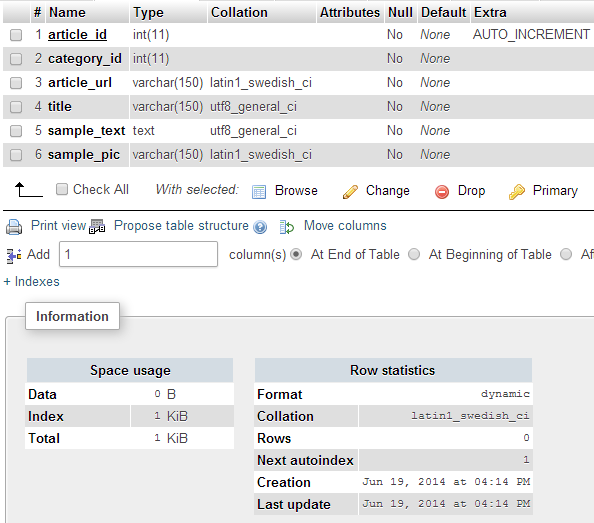
\includegraphics[scale=0.8]{img/article_table}

\vfill

\item{Table \textbf{category:}}\\ \\
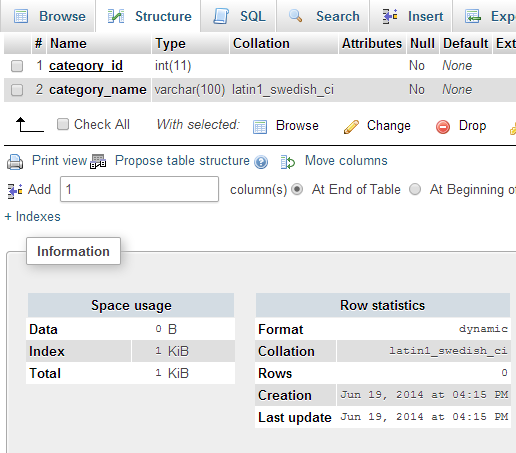
\includegraphics[scale=0.8]{img/category_table}

\vfill

\item{Table \textbf{hit:}}\\ \\
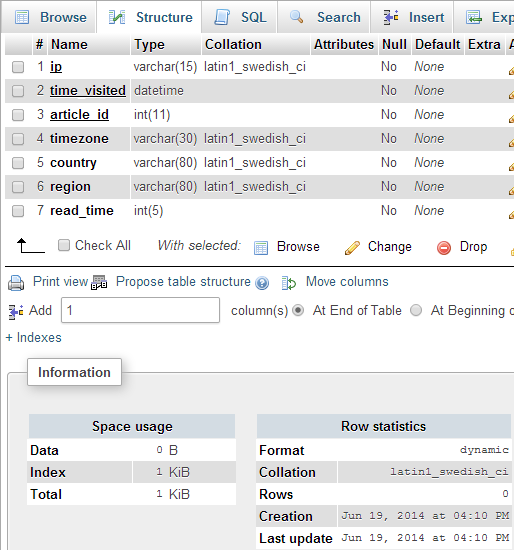
\includegraphics[scale=0.8]{img/hit_table}
\end{enumerate} 

\newpage

\subsection{PHP server-side code}
Now that I created the database, I needed a way to retrieve the data from it. This involved creating configuration files, classes that abstracted the database tables, and code that performed the queries and outputted the resulting data in JSON.
\subsubsection{Configuration and database connection}
First, I created two setup files:
\begin{enumerate}
\item{\textbf{constants.php:}} Holds all the constants that are defined across the application, inclusive of those for the database connection
\item{\textbf{db\_connect.php:}} Performs the PDO database connection based on the given connection parameters
\end{enumerate}
Note that both of these files are stored one directory above \textbf{public\_html/} for security reasons. This folder is called \textbf{lib/}. Thus, the two files are not accessible directly to the public and accordingly need to be included in other PHP files.

\subsubsection{Server-side hit, article, and category capture}
Each table in my database was represented by a PHP class. Hence, the creation of the following 3 classes:
\begin{enumerate}
\item{\textbf{Hit.php:}} This class registers all of the metadata pertinent to a user visit. This data includes IP address, country, region, timezone, and time visited. 
\item{\textbf{Article.php:}} This class captures all of the metadata pertinent to the article being visited. Such includes title, text excerpt, thumbnail URL, and article URL.
\item{\textbf{Category.php:}} This class captures any metadata pertinent to the parent category of the visited article. At the moment, I am only capturing the name of the category.
\end{enumerate}

In addition to the above, I have created a helper file that registers the read time of a given article. By default, the read time is registered as 1 second in the database. Once a hit is registered in the database, the id of the newly created hit is then passed to the DOM of the article page. There, the id is used via an AJAX call to store the calculated read time for the visited article in the database. This file is called \textbf{updateReadTime.php}.
\vfill

\subsection{Client-side read time capture with JavaScript}
As mentioned in the last section, the hit id is passed to the client page in order to keep a way to identify and update the read time for the visited article. Here, I calculated the number of words that are stored in the article. I did this by first getting all of the text found within common article tags - namely <span>, <div>, <article>, <p>, and <section>. I then summed the number of words found within all of the mentioned tags. I ensured that double counting was avoided by using the \textbf{innerText} property; this counted the elements' inner text, but not any text that might have been included in one of its children nodes. Next, I calculated the number of seconds the article was on average expected to take to read. This was based on the human reading speed of 200 words per minute figure that I obtained earlier. This figure was used in the event that a user had left the page open indefinitely. Thus, if an article was expected to take about 5 minutes to read, and the user took (for whatever reason) 30 minutes to navigate away from or to close the article, then I registered the 5 minutes. Although I may have compromised some accuracy here, it remained much more advantageous than having significantly inflated the captured read time.

Once the article page loaded, and the expected read time calculations were made, a timer was readied. The timer was triggered once a user moved the mouse or when the user scrolled the page. This minimized storing metadata created by automated scripts and to a high extent ensured that a human was sitting behind the screen. Upon navigating away from or closing the article, the read time was then submitted to \textbf{updateReadTime.php} and eventually recorded in the database. This part of the implementation relied on the JavaScript events \textbf{window.onbeforeunload} or \textbf{window.onunload}, depending on the browser's user agent. At the time of this writing, this method was tested successfully with Google Chrome 39.0.2171.99 m, Mozilla Firefox 34.0.5, Safari 5.1.7, and Internet Explorer 10.
 
\vfill

\subsection{Tying it all together}
Now that both the back end and front end code has been implemented, I was able to move on to testing this system. I created a miniature lorem ipsum page which acts as an article being visited: \\

\noindent
\includegraphics[scale=1]{img/visit1}

\noindent\ In my PHP code, I populated mock metadata for the article and category. The hit metadata, however, was populated based on the visit data. I went ahead and visited the page for 10 seconds and got the following results:\\

\noindent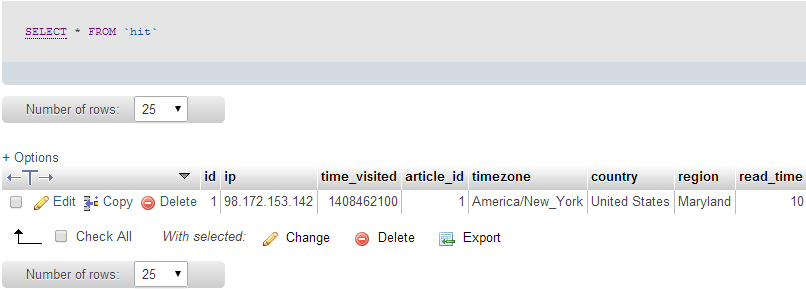
\includegraphics[scale=0.6]{img/visit2}

\noindent\ My ip address, time of visit, article id (at this point a fake one), timezone, country, region, and read time were all stored in the \textbf{hit} table.\\


\noindent\ The article id, category id, article URL, article title, article sample text, and the URL to the article's main pic - were all stored in table \textbf{article}:

\noindent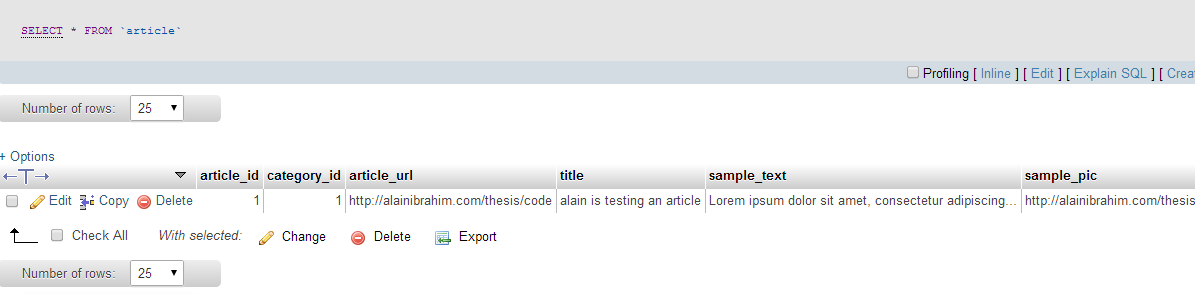
\includegraphics[scale=0.5]{img/visit3} \\

\noindent\ Lastly, the category id and name were both stored in the \textbf{category} table:

\noindent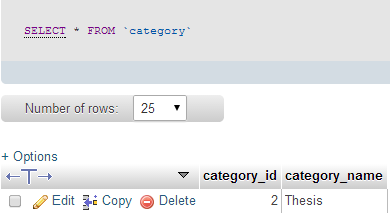
\includegraphics[scale=0.7]{img/visit4} \\


This concludes the part of the system that implements the data capturing. The next step was to connect this library to a working website. For the scope of this thesis, I implemented the hook to specifically tie into a widely used Web Content Management System - Wordpress. 

\newpage

\section{Implementation - hooking into Wordpress}
Wordpress is a web-based Web Content Management System (WCMS). It is essentially a web application that allows its users to create and administer posts, which are ultimately showcased on a website to site visitors. In this project, each news article is implemented as a post and can be categorized under one or more parent categories. Wordpress is very common for its being free and open source; hence, a great candidate for me to test my system against. \\
There is a template file for each post called \textbf{single.php}. This file determines how the article is displayed and what content will be outputted to the visitor. It can be found under the current theme that is being used. A theme in Wordpress is a set of pre-built PHP, HTML, CSS3, and JavaScript templates that structurally and visually dictate how the resultant website looks and behaves. In order to accomplish the task of capturing the data from a certain article, I needed to include my capture library inside \textbf{single.php}. However, since my library cannot directly communicate with Wordpress, I had to create a hook that abstracts some of Wordpress's built-in functions. Lastly, I needed to ensure that Wordpress was using jQuery version 2.1.1 or higher. jQuery is a JavaScript library that shorthands many of the functions needed to interact with the web article's HTML document. Since I needed this library to load before the article page fully loaded, I included jQuery in \textbf{header.php} - which in Wordpress comprises the <head></head> portion of all pages in a given website. 

\newpage 

\subsection{Creating the captureLib folder}
In the interest of portability, I have placed all of my code within a folder called \textbf{captureLib}. If a 3rd party wishes to uses this library in the future, all that would be needed is to simply include \textbf{captureLib} from within \textbf{single.php}. \\


\noindent Below is a breakdown of the current directory structure of the code that captures hits and read times.
\begin{enumerate}
\item \textbf{lib/}
\begin{enumerate}
\item \textbf{constants.php} - contains all the server-side constants that will be used to capture the hits
\item \textbf{db\_connect.php} - connects to the database where the hits are stored
\end{enumerate}
\item \textbf{Article.php, Hit.php, Category.php} - as mentioned previously, these are abstractions of the database tables that communicate the data from and to the database
\item \textbf{getReadTimeLibrary.php} - a line of code to include the read time JavaScript code if a hit was registered
\item \textbf{readTime.php} - this is the JavaScript code that captures the read time. It is terminated with .php (vs. .js) since it requires PHP code to output the hit id inside the JavaScript file. I have made adjustments to this code to accommodate for users switching tabs while reading a certain article. When the article's window loses focus, the timer stops counting; it only resumes when the user gets back to the article window. This maximizes accuracy in the average read time readings.
\item \textbf{wordpressHook.php} - as mentioned earlier, this is an abstraction into Wordpress's needed built-in functions. In order to hook to different CMSs, the code can be modified and reused. 
\item \textbf{countries.php} - contains an array that has all country names. Used for database seeding.
\end{enumerate}

\newpage

\subsection{Creating a mock news website}
In order to test the capture library, I created a mock news site in Wordpress. In this setup, I built the following categories: Business, Entertainment, Music, Science, Sports, Tech, and World. I tasked a friend to populate mock articles with content that is fitting to the parent category. I created the Wordpress install under my personal web hosting account. The URL to it is http://www.alainibrahim.com/fakenewssite. In the interest of time, I used the default theme that came out of the box. \\

\noindent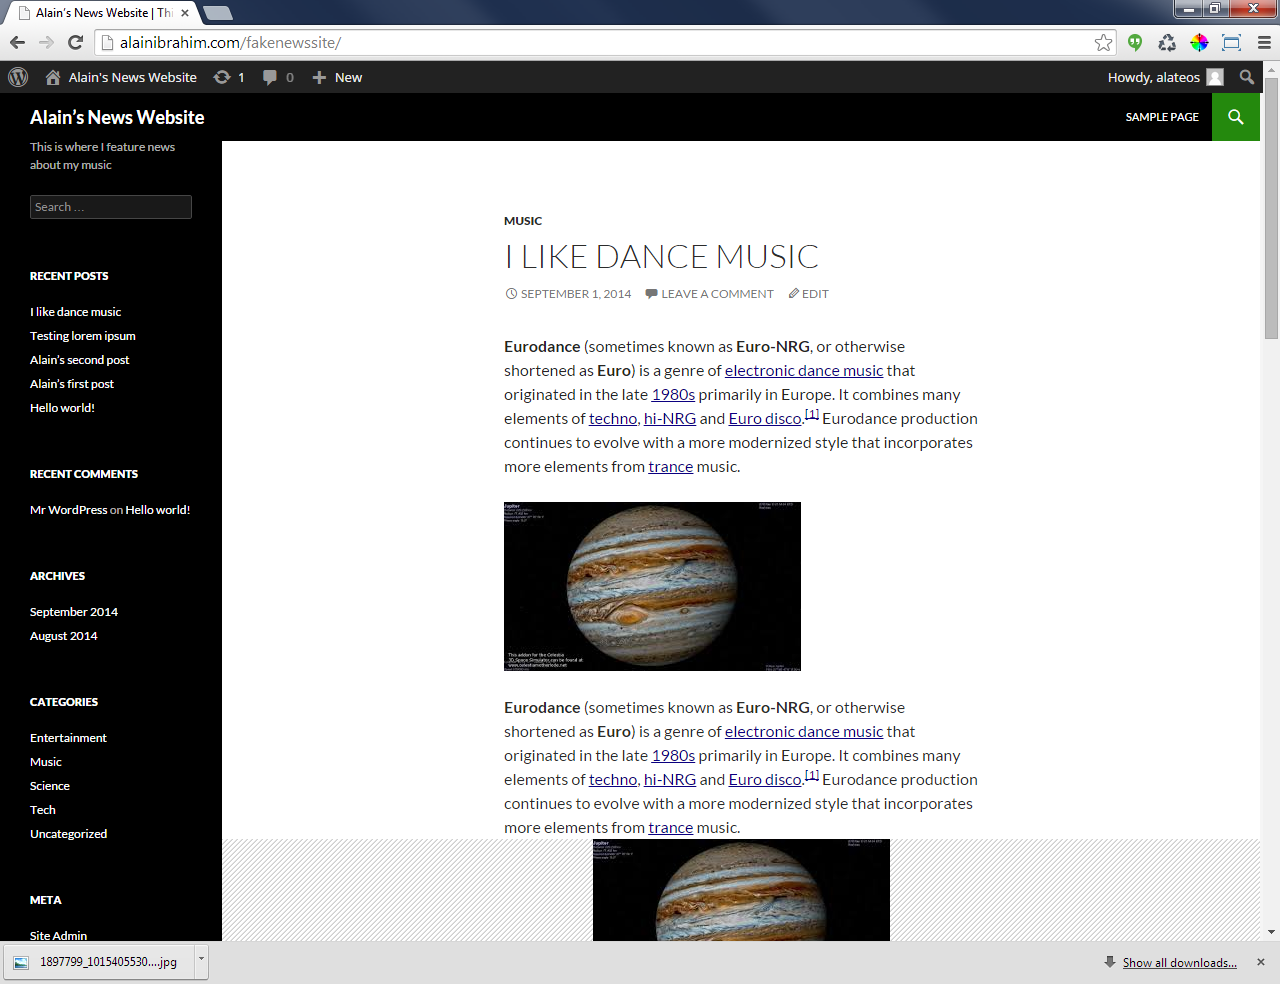
\includegraphics[scale=0.4]{img/fakenewssite_main} 

\newpage

\subsection{Testing}
\subsubsection{Proof of concept}
Below is the result of my having visited 4 different articles, each for a different amount of time:

\noindent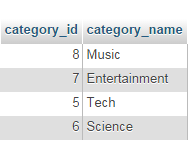
\includegraphics[scale=1]{img/results_categories} \\
\noindent In the \textbf{category} table above, the categories metadata of the different articles that I visited were stored in the database. For this project, I only stored the category's id and name, as they appear in the Wordpress database tables. Note that if I visit an article of the same category again, the category will not be double stored. \\ \\

\noindent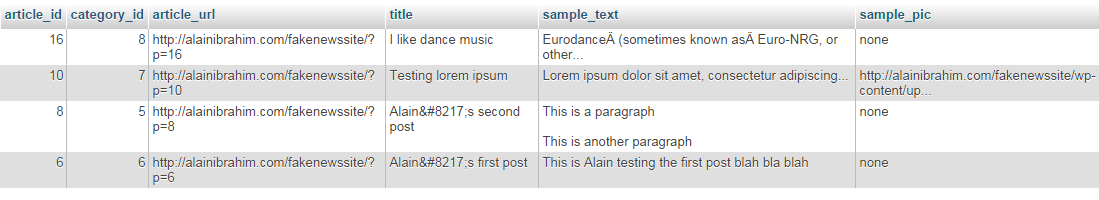
\includegraphics[scale=0.6]{img/results_articles}
\noindent In the \textbf{article} table, the articles' metadata was stored. The sample text is excerpted by PHP with a default setting of 500 characters. This text is later used for previewing articles. \\ \\ 

\noindent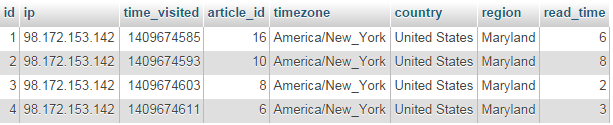
\includegraphics[scale=1]{img/results_hits} \\
\noindent As shown above, the read times (in seconds) appear to have registered successfully in the \textbf{hit} table. 

\subsubsection{Seeding mock data}
After testing the capture of data successfully, I needed a way to mimic traffic on a real news website. In addition, I needed to make it appear as if each mock article visit came from a random country of origin. Below are the steps I took to accomplish this:

\begin{enumerate}
\item{Modified \textbf{constants.php} to include a flag that denotes whether the app is in test or production mode:}
\begin{lstlisting}[basicstyle=\scriptsize]
...

// defines whether we are in test or production mode
define(PRODUCTION_ENV,false);
\end{lstlisting}

\item{Modified class \textbf{Hit.php} to produce a fake read time and fake US state of origin if in test mode:}
\begin{lstlisting}[basicstyle=\scriptsize]
...
// if in test environment, populate fake data for read time and country of origin
if(!PRODUCTION_ENV) {
	// get a random time between 10 seconds and 3 minutes
	$read_time = rand(10,180);
	
	// get the list of all the states in the US, and pick one randomly
	include("states.php");
	$region = $states[array_rand($states)];
}
...
\end{lstlisting} 
\item{Created \textbf{makeFakeHit.php} to invoke a visit to a random article on my fake news site:}
\begin{lstlisting}[basicstyle=\scriptsize]
/**
	The sole purpose of this file is to visit a random article on the 
	fake news site, causing hits to register
*/

$TESTING_IP = "98.172.153.142";

// 290 is the id of the last fake article that was created
$article_id = rand(1,290);

// cause a fake visit only if testing ip address is registered here
if( $_SERVER['REMOTE_ADDR'] == $TESTING_IP) {
	file_get_contents("http://alainibrahim.com/fakenewssite/?p=" . $article_id);
}
\end{lstlisting}
Note that I have hard coded a testing IP address so that I am the only person who can run this for testing. \\
\item{Created \textbf{fakeVisit.html} to run on the client side and to call \textbf{makeFakeHit.php} at a pre-specified time interval(using JavaScript):}
\begin{lstlisting}[basicstyle=\scriptsize]
(function(){
	// the amount of time to wait before revisiting the site (in seconds)
	var REVISIT_INTERVAL = 20;

	// trigger the fake visit on the server side
	var makeFakeHit = function() {
		$.get("makeFakeHit.php");
	}
	
	// set a recurrent loop to seed the data
	setInterval(function(){makeFakeHit();console.log("hit issued")},(REVISIT_INTERVAL*1000));
})()
\end{lstlisting}
\end{enumerate}

\noindent Below is a snapshot of the results of the seeding of the database: \\

\noindent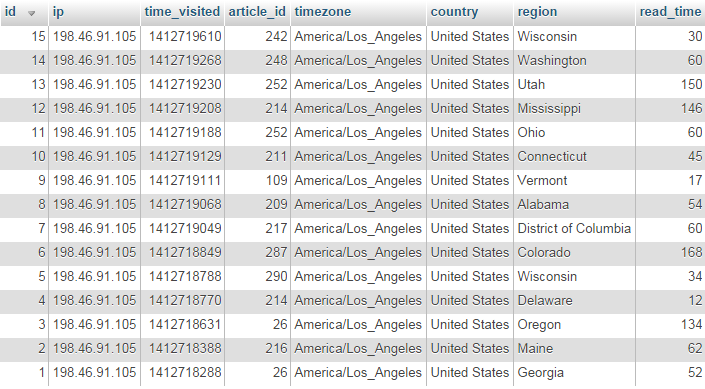
\includegraphics[scale=0.8]{img/seeder_mock_hits} \\

\noindent Note that for each hit, the data that is generated by the seeding process is \textbf{article\_id}, \textbf{region}, and \textbf{read\_time}.

\newpage

\section{Implementation - retrieving captured metrics}
At this point, the database was populated with a good amount of data and I needed a way to retrieve it. For this, I created a folder on the server side and called it "vizLib". In this directory I created 3 PHP files that outputted the results in JSON:
\begin{enumerate}
\item{\textbf{getCategories.php} - outputs all the used article categories.}

\item{\textbf{getCategoriesMetrics.php} - outputs all of the metrics for all categories.}

\item{\textbf{getArticlesMetrics.php} - outputs all of the metrics for all the articles given a category ID, beginning visit time, and ending visit time.}

\item{\textbf{getArticleCountriesMetrics.php} - outputs all of the country metrics for a given article ID.}

\item{\textbf{index.php} - the landing page for the visualization}

\end{enumerate}

\newpage

\section{Implementation - visualization}

This brings us to the final piece of the project - conveying the web traffic to the visitor with an interactive and navigable visualization. \\ As mentioned earlier, the goal of the visualization was to support the following tasks:
\begin{enumerate}
\item To compare articles' hits and reader attention spans for any period within the last month, given a select category
\item To preview each article's thumbnail, title, and excerpt
\item To contrast the geographic distribution of hits and attention of up to 2 articles
\item To navigate to the full article counterpart on the subject news website
\end{enumerate}

\subsection{The controls box}

The controls box helped the visitors filter the news categories and time range of the articles hits. Typically, controls take up space in the limited real estate area available in any web browser. Though, I felt it would be best to allocate this space to the visualization. For this reason, I made the controls box drag-able and hide-able.

\noindent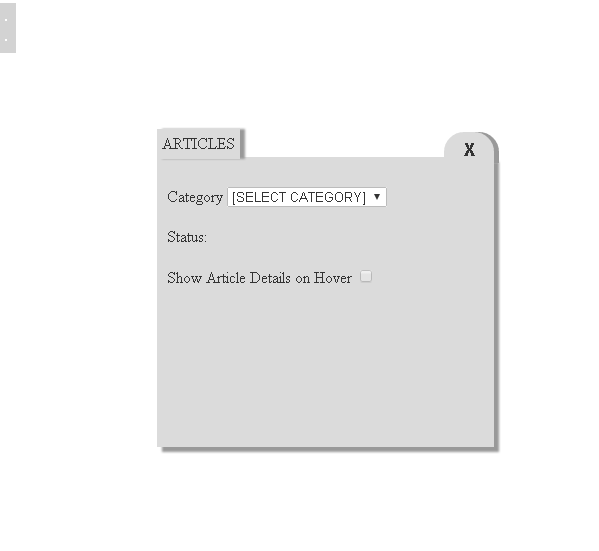
\includegraphics[scale=0.8]{img/viz_3}

\noindent The controls box first partially loads when no category is selected. The "X" hides it; when this is done, the top left gray rectangle with the two white dots is then contoured by a black border - to indicate that it is hidden.

Upon loading the visualization, an AJAX call is made to the server which fetches all the of the news categories into this dropdown box. Once a category is selected, a call is made to the server, which results in all of the data for the selected category to be fetched from the database using the server-side script.\\ \\ The user is notified (via the red colored "Loading..." indicator) of when the data is being loaded for a news category:

\noindent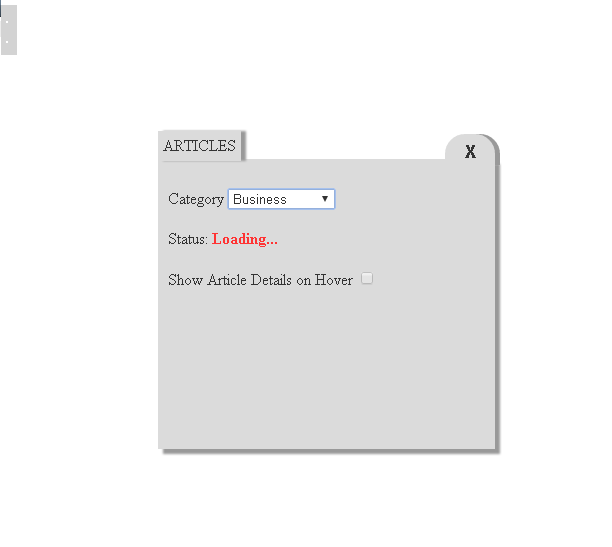
\includegraphics[scale=0.6]{img/viz_4}

And, once the data is loaded, the status label turns green and reads "Loaded":

\noindent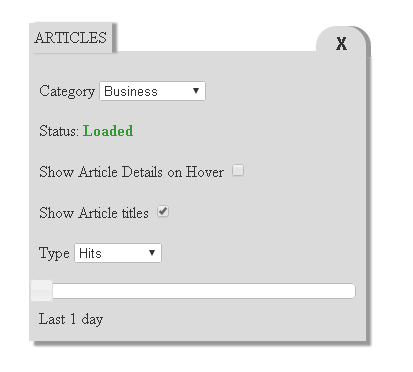
\includegraphics[scale=0.6]{img/viz_5}

\newpage

\noindent Below are the descriptions for each component of the controls box:

\begin{itemize}
\item \textbf{Category - } sets the category whose articles the user chooses to see
\item \textbf{Status - } shows the data transfer status of the selected news category
\item \textbf{Show Article Details on Hover - } determines whether a preview of the article will pop up upon hovering over an article in the stacked area chart. 
\item \textbf{Show Article titles - } toggles the visibility of the article titles in the bottom portion of the screen
\item \textbf{Type - } the user gets to select between viewing the number of hits or amount of time spent (in seconds) on the Y axis of the stacked area chart
\item \textbf{Time slider - } This is a dual time slider control in that the user can use it to select one slice (i.e. day) in time or can alternatively select a time range to view the data in 
\end{itemize}

\newpage

\noindent I made the controls box transparent in case the user wants to keep it afloat the visualization: \\

\noindent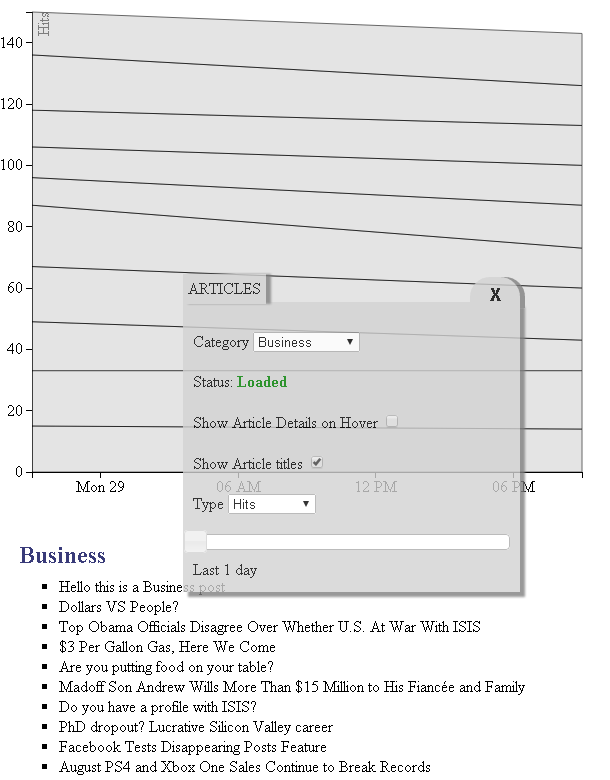
\includegraphics[scale=0.8]{img/viz_6}



\subsection{The Stacked Area Chart}

Here, the goal was to create a visual product that would allow the user to view all the articles' popularity over time, given a certain news category. I knew that I wanted time to go on the horizontal X axis, and hits or read time to go on the Y axis. Based on this, I first started with a simple line graph, where each line represented an article that was colored differently from the other lines. There were 2 downsides which led me to abandon the line graph: 
\begin{itemize}
\item The lines intersected into a spaghetti mash-up, making it very difficult to spot any significant patterns
\item When a category (e.g. Business) contained more than 8 articles, I had to use 8 different colors to encode the articles. The issue here was that at a certain point, colors became very similar making it almost impossible to visually follow the article all the way through a selected time period 
\end{itemize}

\noindent I instead used the stacked area chart. The stacked area chart maintained a view on the patterns without compromising legibility and supported the following tasks: 
\begin{itemize}
\item To compare articles' hits and reader attention spans for any period within the last month, given a select category
\item To preview an article's thumbnail, title, and excerpt
\end{itemize}

\noindent The X axis is laid out using D3 and represents time aggregated on an hourly basis: 

\noindent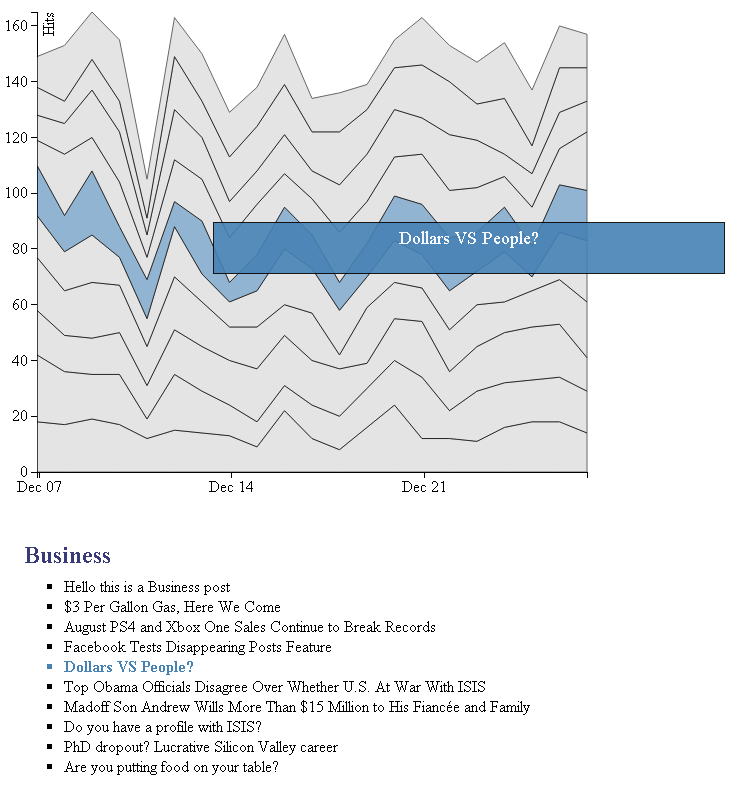
\includegraphics[scale=0.8]{img/viz_1}

The articles are stacked vertically, each respectively matching its title in the below white space area, which is headed by the selected category. The readying of the data for the stack is done using the D3 area layout, and the visual representation is implemented by using the SVG <path>. The paths by default all contain a fill of light gray. 

Hovering over any article in the stack chart causes both the article's area and corresponding title to turn to steel blue. In reverse, hovering over an article title in the bottom area causes the corresponding article's area in the stack chart to have a fill color of steel blue. 
It is important to note that the user has the option to see a preview of the selected article when checking "Show Article Details On Hover" in the controls box:

\noindent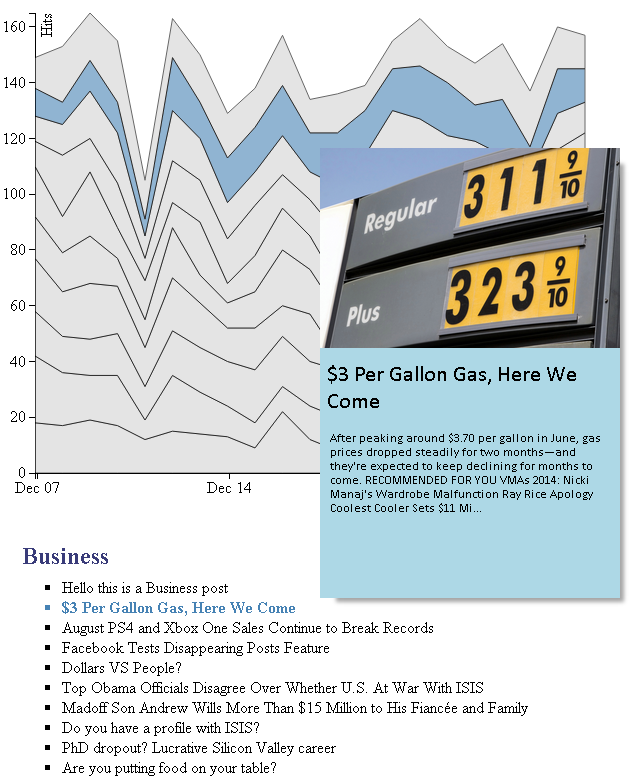
\includegraphics[scale=0.7]{img/viz_2} \\

This results in an overlay to pop over the selected article that includes the article's thumbnail, title, and a 500-character excerpt of the body of the article. 

The user is given the option to contrast the pattern of up 2 articles over time, by left clicking on the select article area. This results in one article being filled with a purple color and the other with a green color. I picked the colors from colorbrewer2.org and ensured they were colorblind safe.

\noindent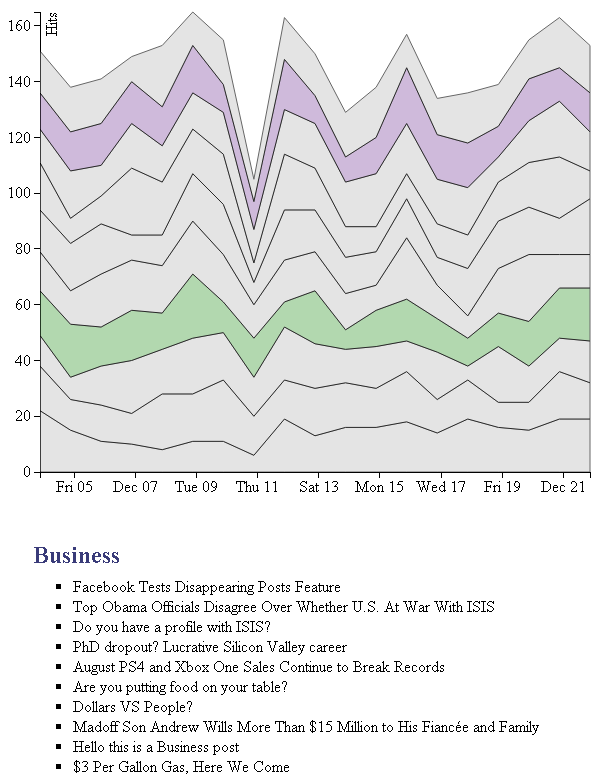
\includegraphics[scale=0.8]{img/viz_7} \\

\noindent Once the two articles are selected, their corresponding geographic distributions are shown in the right area of the browser. This is covered in the next section. 

\newpage

\subsection{Geographic bar charts}

In the previous section, two articles are clicked on in the stacked area chart. In addition to their being highlighted in the stacked area chart, a right side pane populates each article's title in its color, along with a table below it. The table contains the geographic origin (e.g. state/country), the total number of hits, and the attention span distribution (i.e. read time in seconds).\\

\noindent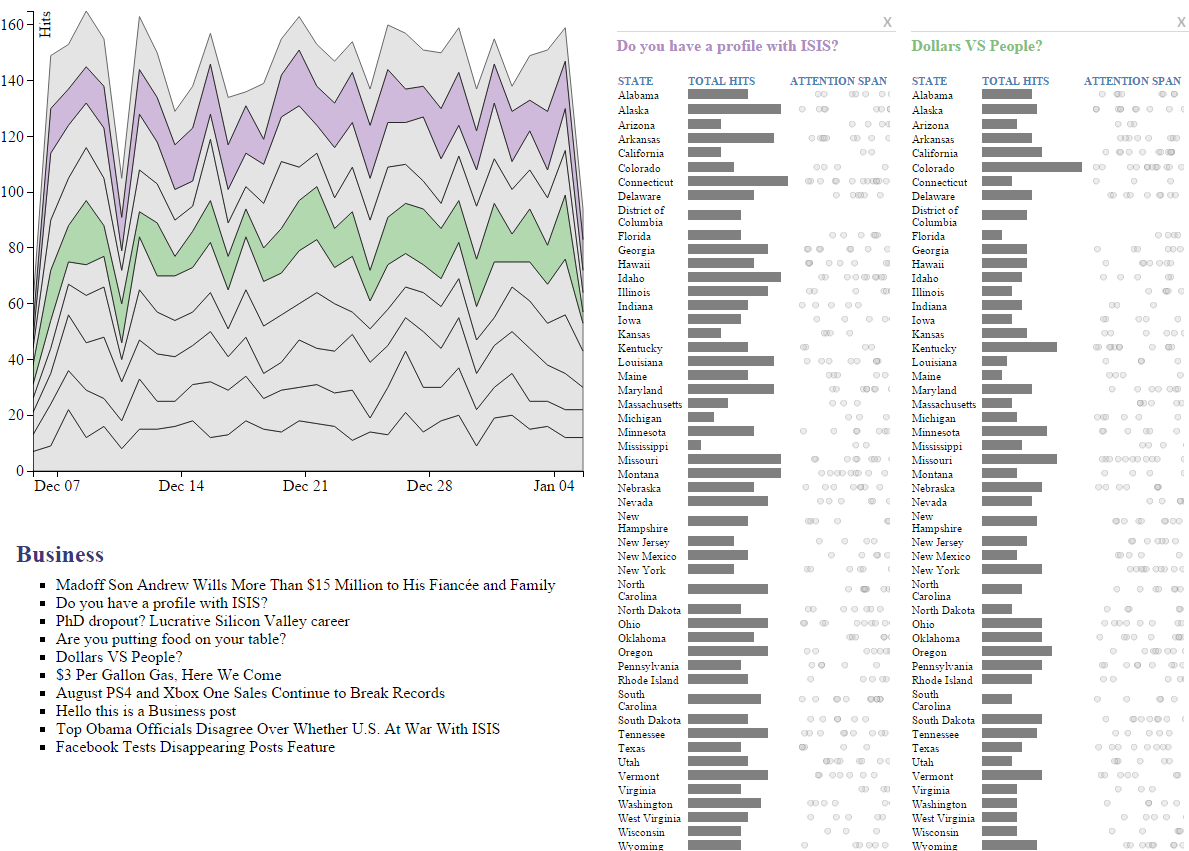
\includegraphics[scale=0.5]{img/viz_8} \\

Whenever a first article is selected, the second article is compared along the same geographic areas for uniformity. That is, only the geographic areas that are included in the first article are displayed for the second article. Clicking the top right "X" removes the article from the right pane, and renders the graph area counterpart back to light gray. 
The hits values are encoded as horizontal bars in dark gray. The attention span column contains a distribution of the captured read times, represented as light gray circles; the amount of seconds spent is encoded by the horizontal position of each circle. The circles are transparent to allow for overlap. The maximum horizontal position of the circle is demarcated by the expected read time. The expected number of seconds was discussed earlier, and is a measure that takes into account the average adult human reading speed and the number of words contained within the article. The total hits bar spans relative to the highest hits value for that article - meaning, the bar that takes up the biggest width is the highest hit value that was registered for that article. 

\vfill

\noindent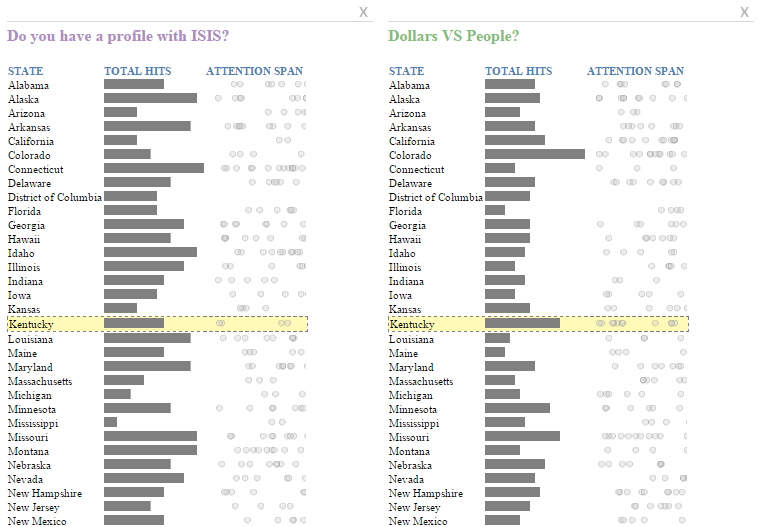
\includegraphics[scale=0.8]{img/viz_9} \\

\noindent We now examine the geographic area in more detail. Note that automatically, the entries are sorted by the name of the geographic origin, in ascending order. Clicking on the "STATE" header toggles back and forth the sorting order of the geographic origin name. Similarly, toggling the "TOTAL HITS" header sorts the data in ascending/descending order. When the data is sorted, it is sorted according to the same criterion for both articles. Hovering over a row will cause that row to be highlighted in yellow, and to be contoured in a dashed line solid border. Hovering over any bar will in addition pop up a steel blue overlay which displays - using white text - the number of hits or read time in seconds.  

The geographic bar charts support the following tasks:
\begin{itemize}
\item To contrast the geographic distribution of hits and attention of up to 2 articles
\item To navigate to the full article counterpart on the subject news website
\end{itemize}

\newpage

\section{Results}

\subsection{Mock Website}
The working example that I have discussed so far is based on a mock website that I created using mock visit data.

\subsubsection{Capturing Web Metrics}
\begin{itemize}
\item For each hit, the following metadata was successfully captured: IP address, time visited, article ID, time zone, country of origin, and region of origin
\item For each hit, the read time was captured as a random number between 10 and 180 seconds. When I switched the flag in my PHP code to denote the production environment, the read time was captured successfully when I navigated away from a news article. Most of my testing was done in Google Chrome version 39
\item Each hit was captured according to the revisit threshold time (in seconds) that was specified in the PHP code
\item Each category was captured from Wordpress via the PHP libraries I created
\item Each article's metadata was captured from Wordpress via the PHP libraries I created
\end{itemize}

\subsubsection{Retrieving Web Metrics}
\begin{itemize}
\item The categories were successfully retrieved in JSON via \textbf{getCategories.php}
\item The hits data was retrieved successfully from the MySQL database using JSON via \textbf{getArticlesMetrics.php}. I initially reserved the geographic data for the articles to be serviced by \textbf{getArticleStatesMetrics.php}. However, I felt that in a production environment that many SQL calls to the database server would slow down the system and affect all users. In order to minimize the number of requests to the server, I had the server fetch all data for a given category for the last 31 days. The client-side JavaScript code then parsed and re-organized the fetched data to be used by the interactive visualization
\end{itemize}

\subsubsection{The Interactive Visualization}
\begin{itemize}
\item The final product included a stacked area chart, a list of article titles below, and a right pane for geographic analysis of up to 2 articles
\item The hits were first aggregated on a minute to minute basis. This resulted in performance degradation. Adjusting the date range took a delay of about 2-3 seconds to reflect in the redraw of the stacked area chart. I then aggregated on an hourly basis, which ended up plotting Y values over 744 (31 days x 24 hours) X axis time values. This eliminated the delay in the stacked area chart redraw
\item The stacked chart accurately reflected the number of hits and average read time over the selected time range
\item Clicking one or more articles highlighted the article area in the stacked area chart and displayed the total hits based on geography. It also showed the distribution of the recorded read times. For the mock site, the geography was limited to states within the United States
\item The tables that contained the geographic origins were sortable by total hits and by state name - in ascending and descending order
\item When "Show Article Details on Hover" was enabled, the pertinent article's thumbnail image, title, and body excerpt were successfully presented in an overlay
\item Hovering over any row in the geographic hits and attention span table resulted in the row being highlighted in yellow for all articles that are being compared
\item Hovering over a bar representation of the total number of hits invoked a steel blue overlay showing the number of hits
\\
\noindent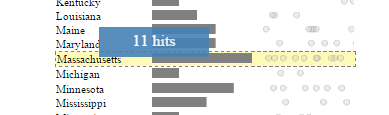
\includegraphics[scale=0.8]{img/state_hit_hover} \\  

\item Hovering over an attention span circle invoked a steel blue overlay showing the number of seconds that was spent on the article
\noindent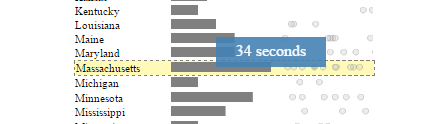
\includegraphics[scale=0.8]{img/state_circle_hover} \\  
\end{itemize} 

\subsubsection{Performance}
\begin{itemize}
\item In the mock site, the last 31 days amounted to ~4500 hits per category. The time it took for them to be loaded in the visualization was around 4 seconds, using a PC with an Intel i7 processor and 12 GB of RAM
\item When changing the date range, the stacked chart's redraw time was almost instantaneous. Again, using a PC with an Intel i7 processor and 12 GB of RAM
\item When "Show Article Details on Hover" was enabled, there was a delay of about 500 milliseconds for the image thumbnails to initially show. Once they were cached in the browser's memory, they appeared without delay. For images that were not cached, the delay was about 1 second per megabyte in picture size
\end{itemize}

\newpage

\subsection{Actual Website}
Being a web developer at a news organization, I was able to test the system against one of our mini sites - Afia Darfur (http://www.afiadarfur.com), since it was using Wordpress as its back-end platform. The site targets visitors from Sudan and keeps them up to date with news specific to Sudan. \\

\noindent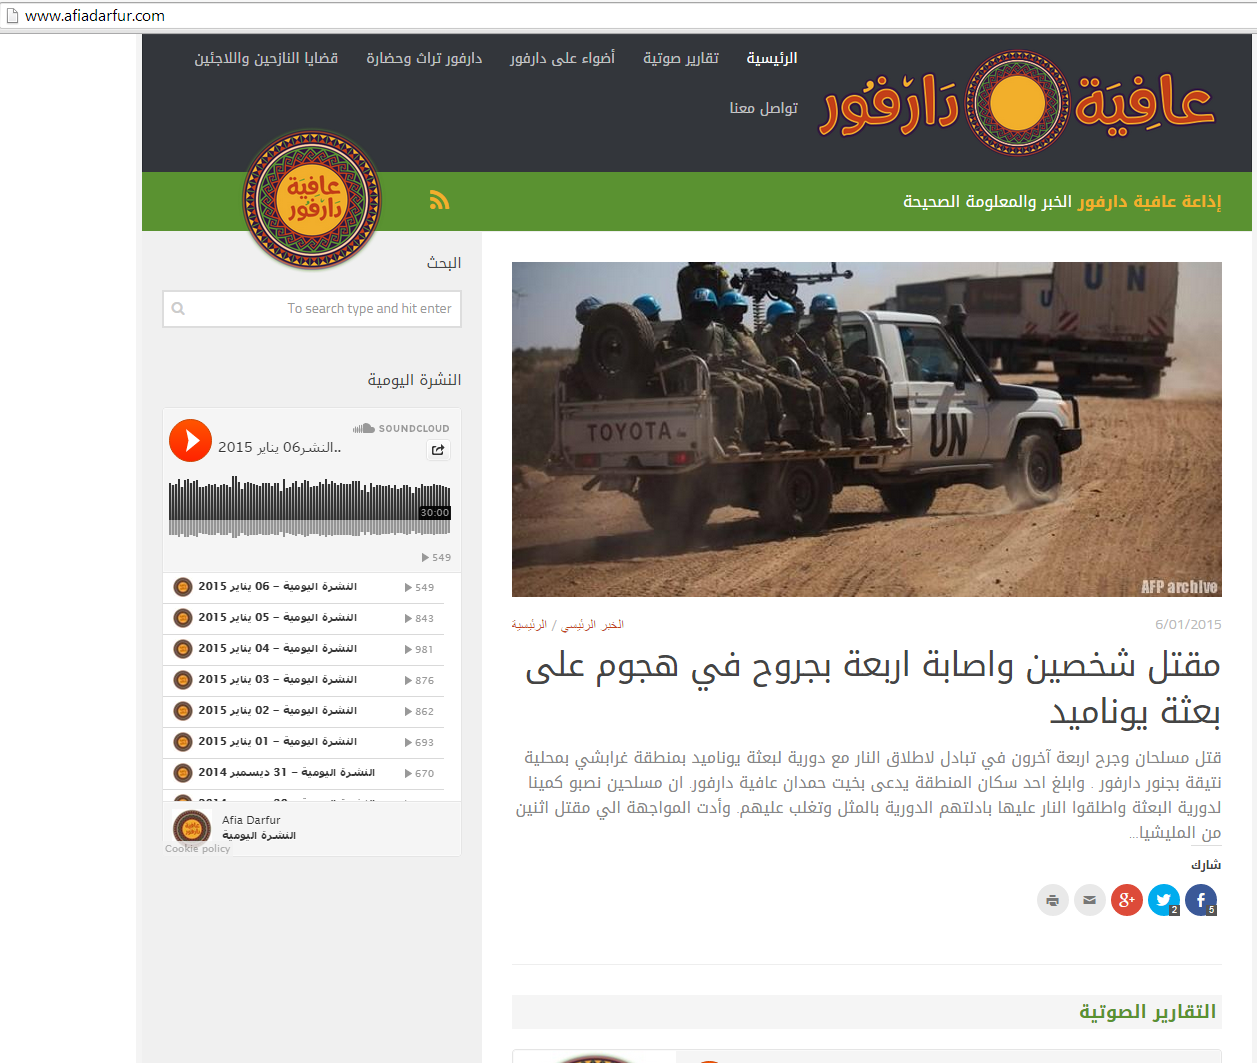
\includegraphics[scale=0.4]{img/afiadarfur_main} \\

\subsubsection{Hooking the Custom Libraries into Afia Darfur}
Hooking into the live website involved the following steps:
\begin{enumerate}
\item Creating a database for the web metrics
\item Placing the \textbf{captureLib/} folder in the root folder of the Wordpress theme
\item Including the capture library in Wordpress's \textbf{single.php} 
\item Including the \textbf{vizLib/} folder in the root directory of the website
\item Placing \textbf{updateExpectedReadTime.php} and \textbf{updateReadTime.php} in the root directory of the website 
\end{enumerate}

\subsubsection{Capturing Web Metrics}
\begin{itemize}
\item For each hit, the following metadata was successfully captured: IP address, time visited, article ID, time zone, country of origin, and region of origin
\item  The read time was captured successfully when I navigated away from a news article. Most of my testing was done in Google Chrome version 39
\item Each hit was captured according to the revisit threshold time (in seconds) that was specified in the PHP code. For Afia Darfur, this was set to 20 seconds
\item Each category was captured from Wordpress via the PHP libraries I created
\item Each article's metadata was captured from Wordpress via the PHP libraries I created. In order to ensure that the Arabic text was captured, I had to change the collation of the database tables to utf8\_general\_ci
\item The PHP library files responsible for capturing data had to be encoded in UTF-8
\end{itemize}

\subsubsection{Retrieving Web Metrics}
\begin{itemize}
\item The categories were successfully retrieved in JSON via \textbf{getCategories.php}. The pertinent PHP files had to be encoded in UTF-8 to handle the Arabic characters
\item The hits data was retrieved successfully from the MySQL database using JSON via \textbf{getArticlesMetrics.php}. I initially reserved the geographic data for the articles to be serviced by \textbf{getArticleStatesMetrics.php}. However, I felt that in a production environment that many SQL calls to the database server would slow down the system and affect all users. In order to minimize the number of requests to the server, I had the server fetch all data for a given category for the last 31 days. The client-side JavaScript code then parsed and re-organized the fetched data to be used by the interactive visualization
\end{itemize}

\subsubsection{Visualization The Web Metrics}
\begin{itemize}
\item The final product included a stacked area chart, a list of article titles, and a right pane for geographic analysis of up to 2 articles
\\ \\
\noindent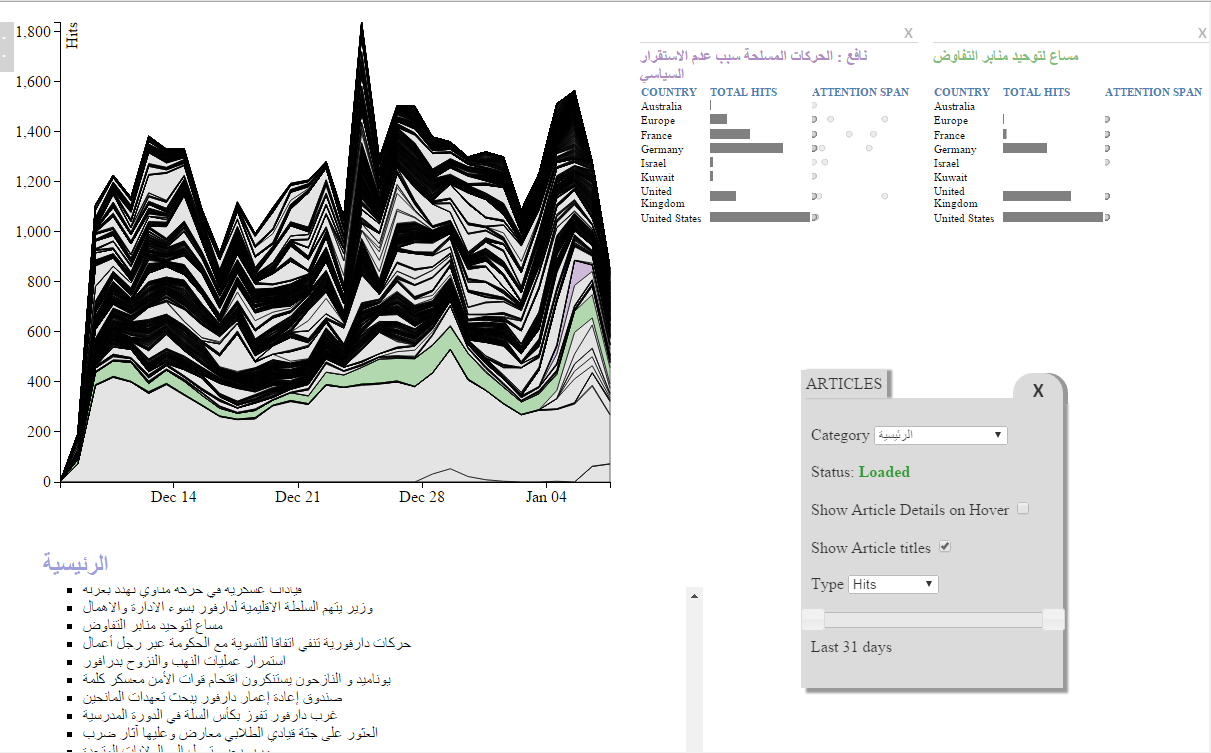
\includegraphics[scale=0.5]{img/afiadarfur_main_viz} \\
\item The hits were aggregated on an hourly basis resulting in Y values over 744 (31 days x 24 hours) X axis time values
\item The stacked chart accurately reflected the number of hits and average read time over the selected time range
\item Clicking one or more articles highlighted the article encode in the stacked area chart and displayed the total hits based on geography. It also showed the distribution of the recorded read times. Since the target audience of Afia Darfur is an international one, the geographic data was aggregated to countries - unlike in the mock site where units of geography were represented as US states
\item The tables that contained the geographic origins were sortable by total hits and by state name - in ascending and descending order
\item When "Show Article Details on Hover" was enabled, the pertinent article's thumbnail image, title, and body excerpt were successfully presented in an overlay \\ \\
\noindent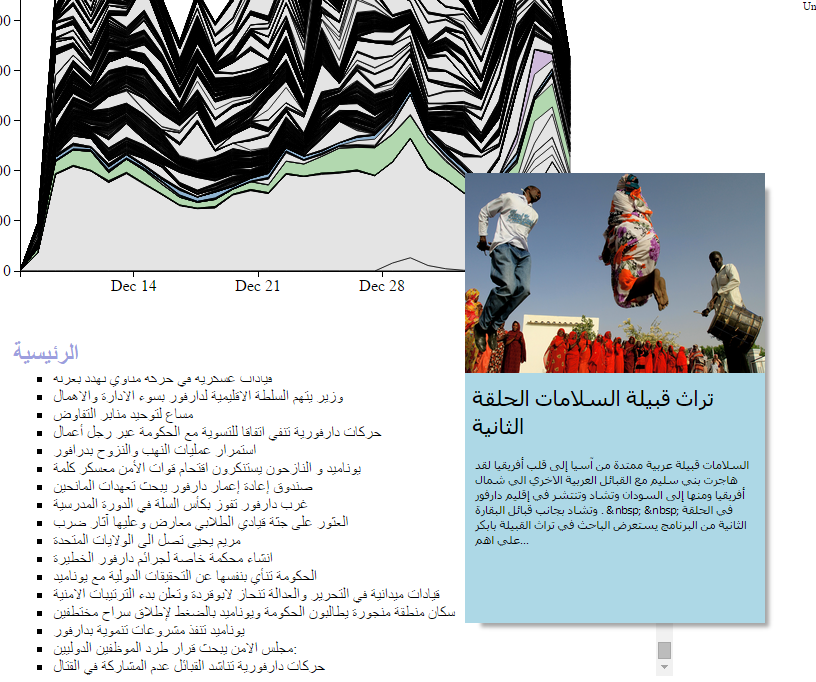
\includegraphics[scale=0.5]{img/afiadarfur_hover} \\
\\
\item Hovering over any row in the geographic hits and attention span table resulted in the row being highlighted in yellow for all articles that are being compared
\item Hovering over a bar representation of the total number of hits invoked a steel blue overlay showing the number of hits 
\\
\noindent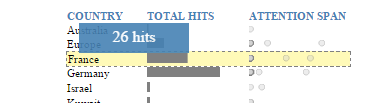
\includegraphics[scale=0.8]{img/country_hit_hover} \\  
\item Hovering over an attention span circle invoked a steel blue overlay showing the number of seconds that was spent on the article
\\
\noindent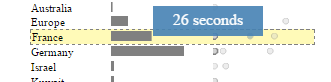
\includegraphics[scale=0.8]{img/country_circle_hover} \\   
\end{itemize} 


\subsubsection{Performance}
\begin{itemize}
\item In the Afia Darfur website, the last 31 days amounted to ~10,000 hits and ~40,000 hits for the two main categories being used by the web editors. It took approximately 16 seconds to load the ~10,000 hits and 52 seconds to load the ~40,000 hits. 
\item As for adjusting the stacked area graph's time range, there was a ~3-second delay for the ~10,000 hits and a ~10-second delay for the ~40,000 hits. This was done using a PC with an Intel i7 processor and 12 GB of RAM. 
\item When "Show Article Details on Hover" was enabled, there was a delay between 50 to 300 milliseconds for the image thumbnails to initially show. Once they were cached in the browser's memory, they appeared without delay. For images that were not cached, the delay was about 1 second per megabyte in picture size
\end{itemize}

\newpage

\section{Conclusion}
My research on visualizing data coupled with my programming and relational database development experience resulted in the implementation of a  MySQL relational database to house the web traffic metrics, a capture and visualize PHP code library, and an interactive web-based visualization. This system worked best when web editors placed their articles under several categories.  \\ 

In order to test the implemented library, I built a mock news website in Wordpress. I then built a script that mimicked random visits to the mock articles every 20 seconds. Since I could not mimic an actual visit where the user scrolls the article and where the read time is captured upon the user navigating away, I created an automated script that seeded a random time between 10 seconds and 2 minutes for each visit. \\ When I hooked my library into the mock website, the web metrics were captured as intended. 
In the final step, I implemented the interactive web-based visualization using JavaScript. The visualization supported the tasks it was designed to enable. \\

Next was the step of testing with a live Wordpress-based website. I hooked the capture and visualize library to Afiadarfur.com, a website geared to presenting new from Sudan. The capture code registered the hits into the MySQL database. Not all read times were registered for the article visits due to factors such as older web browsers not supporting the \textbf{onunload()} method, and due to JavaScript plugins that may have conflicted with the capture library. Though, the the read times that were successfully captured were accurate. 
  
As for the interactive visualization for Afiadarfur.com, the stacked area chart showed around 300 stacked areas for one of the main news categories, which resulted in a considerable latency between changing the date range values in the filter controls box and in seeing the visual update of the chart. This was the result of the web editors categorizing most of their articles under 2 main categories, each which had a high concentration of articles. Thus, for the stacked area chart to work efficiently, editors needed to spread their articles under several categories such as business, music, world, and entertainment. Doing this across several categories would have greatly reduced the latency. Another implementation measure that could have decreased latency would have been to add more filters - or, to narrow the maximum time window into the hits data to about 1 week. 
Showing the geographic distribution of hits and read times between two articles was successful. Aggregating the data on an hourly basis resulted in a low visual latency, while maintaining temporal accuracy. \\

Overall, the resultant interactive visualization successfully conveyed patterns of articles' popularity and levels of interest for each article - all while allowing the visitor to preview every article and navigate to its website post.

\newpage

\section{Future Work}
I would have liked to add the following capabilities to my existing visualization:
\begin{itemize}
\item To create a stacked area chart for categories over time, similar to the existing one for articles
\item To visualize each article's interest fluctuations as a relative measure from its publication date. In the current scenario, one is able to see which articles peak and plunge over time. However, it is difficult to contrast two or more articles' fluctuations since their inception date
\item To allow for 4 articles to be simultaneously contrasted across their geographies. I can accomplish this by removing the attention span column and having it as a filter option to narrow the geographic tables
\item To visualize the number of hits and attention spans per capita
\item To capture social media metrics such as Facebook likes and  Twitter tweets, and incorporate them into the stacked area chart 
\item To cache the IP addresses of the visitors in order to minimize calls to the 3rd party API Telize.com
\item To cache query results for each category so as to minimize the request load on the database server
\item To capture each a hit via a token stored in HTML5's \textbf{LocalStorage} array. In this scenario, if two people visiting the same article are behind the same IP address, then they would be counted as 2 separate hits versus 1 hit. Here, if the user decided to disable JavaScript, I could then fall back onto the method I implemented in this thesis - which is identifying each hit as coming from a unique IP address
\end{itemize}
\newpage

\section{Glossary}
\begin{itemize}
\item[] \textbf{Apache HTTP Server (aka Apache)}: A web server software program
\item[] \textbf{Choropleth map}: A thematic map in which areas are shaded or patterned in proportion to the measurement of the statistical variable being displayed on the map (source: Wikipedia).
\item[] \textbf{Class}: In object oriented programming parlance, it refers to the abstraction and representation of a real life object or concept in code.
\item[] \textbf{CSS}: A styling language used to define the aesthetics of elements in a web deliverable. This is implemented in all major web browsers. CSS3 is the most recent version of this language.
\item[] \textbf{D3.js}: A JavaScript library for manipulating documents based on data using HTML, SVG and CSS (source: d3js.org).
\item[] \textbf{Google Analytics}: A service offered by Google that generates detailed statistics about a website's traffic and traffic sources and measures conversions and sales (source: Wikipedia).
\item[] \textbf{HTML 5}: The most recent specification for the markup language that constitutes the visual elements of any web deliverable. It also normally includes some JavaScript and CSS 3 code as part of its implementation.
\item[] \textbf{JavaScript}: A client-side scripting language that is used by all prominent web browsers.
\item[] \textbf{JSON (JavaScript Object Notation)}: A lightweight data-interchange format (source: json.org).
\item[] \textbf{LAMP}: A web development environment comprised of a Linux server, Apache HTTP Server, MySQL, and PHP.
\item[] \textbf{MySQL}: An open source relational database management system.
\item[] \textbf{Object oriented programming}: A programming paradigm that represents real-life elements and concepts as "objects". The implementation involves mimicking only the needed real-life characteristics of the object in code, and calling a working copy of these objects an "instance".
\item[] \textbf{PHP}: An open source server-side scripting language.
\item[] \textbf{Relational database}: A database built on principles of the relational model. Such a database is comprised of tables and fields.
\item[] \textbf{SVG}: An XML-based vector image format for two-dimensional graphics that has support for interactivity and animation (source: Wikipedia).
\item[] \textbf{Web visualization}: A visual deliverable created using web technologies. More than often, it is dynamic in that it visually changes based on the data being fed to it. 
\end{itemize}

\vfill

\begin{thebibliography}{1}

  \bibitem{schumann} Schumann, H. and Muller, W. (2000). {\em Visualisierung - Grundlagen und allgemeine Methoden}. Springer, Berlin, Germany.

  \bibitem{tufte}  Tufte, E.R. (2001). {\em The Visual Display of Quantitative Information} (2nd ed.) Cheshire, CT: Graphic Press.

  \bibitem{munzner} Munzner, T. (2009), {\em A Nested Model for Visualization Design and Validation}. Retrieved from \\ https://www.cs.ubc.ca/labs/imager/tr/2009/NestedModel/NestedModel.pdf

  \bibitem{cockburn} A. Cockburn, A. Karlson, A.K., \& Bederson B.B.(2008). {\em A review of overview+detail, zooming, and focus+context interfaces.} ACM Computing Surveys (CSUR), vol. 41, no. 1, pp. 1-31. New York, NY: Association for Computing Machinery, Inc.
  
  \bibitem{playfair} Playfair,W. and Corry, J. (1801). {\em The Commercial and Political Atlas: Representing,
by Means of Stained Copper-Plate Charts, the Progress of the Commerce,
Revenues, Expenditure and Debts of England during the Whole of
the Eighteenth Century} (3rd ed.). London, United Kingdom: Wallis.
  
  \bibitem{frank} Frank, A. U. (1998). Different Types of "Times" in GIS. In Egenhofer, M. J.,
\& Golledge, R. G., (Eds.), {\em Spatial and Temporal Reasoning in Geographic
Information Systems}, pp. 40-62. New York, NY: Oxford University Press.

  \bibitem{goralwalla} Goralwalla, I. A., \"{O}zsu, M. T., \& Szafron, D. (1998). An Object-
Oriented Framework for Temporal Data Models. In Etzion, O., et al., (Eds.), {\em Temporal Databases: Research and Practice}, pp. 1-35. Berlin,Germany: Springer.
  
  \bibitem{bettini} Bettini, C., Jajodia, S., \& Wang, X. S. (2000). {\em Time Granularities in
Databases, Data Mining, and Temporal Reasoning} (1st ed.). Secaucus, NJ: Springer.

  \bibitem{radner} Radner,W., Diendorfer, G., (2014). English sentence optotypes for measuring
reading acuity and speed - the English version of the Radner Reading Charts.
{\em Charts Graefe's Archive for Clinical and Experimental Ophthalmology}, 252 (8), 1297-1303. Berlin; New York: Springer-Verlag.

  \bibitem{wills} Wills, G., (2011). {\em Visualizing time: Designing Graphical Representations
for Statistical Data} (1st ed.). New York: Springer.

  \bibitem{clevelandmcgill} Cleveland, \& W., McGill, R., (1984). Graphical perception: Theory,
experimentation, and application to the development of graphical methods. {\em Journal of the American Statistical Association}, 79 (387), 351-354.
  
  \bibitem{colinware} Healey, C.G., (1996). Choosing effective colours for data visualization. {\em Proceedings of the 7th conference on Visualization} '96, 263-270. Los Alamitos, CA: IEEE Computer Society Press. 
  
  \bibitem{byronwattenberg} Byron, L., \& Wattenberg, M., (2008). Stacked Graphs - Geometry \&
Aesthetics. {\em EEE Transactions on Visualization and Computer Graphics Archive}, 14 (6), 1245-1252. Piscataway, NJ: EEE Educational Activities Department.

  \bibitem{swires} Swires-Hennesy, E., (2014). {\em Presenting Data: How to Communicate Your Message Effectively}. West Sussex, United Kingdom: John Wiley \& Sons Ltd.
  
  \bibitem{codd} Codd, E.F. (1970). A Relational Model of Data for Large Shared Data Banks.
{\em Communications of the ACM}, 13 (6), 377-387. New York, NY: Association for Computing Machinery, Inc. 

  \bibitem{carpendale} Carpendale, M. S. T. (2003). {\em Considering visual variables as a basis for information visualisation}. Computer Science TR\# 2001-693, 16.   
  
  \end{thebibliography}
 


\end{document}
